\documentclass[a4paper]{article}

\usepackage[utf8]{inputenc}
\usepackage[T1]{fontenc}
\usepackage{tikz}
\usetikzlibrary{shapes.geometric, arrows.meta, positioning, fit, backgrounds, calc, decorations.pathreplacing}
 
\usepackage{pdp}
\usepackage{subcaption}
\usepackage{float}
\usepackage{listings}
\usepackage{xcolor}
\usepackage{tikz}
\usepackage{amssymb}
\usetikzlibrary{positioning, shapes, arrows.meta}
\usepackage{hyperref}
\usepackage{tabularx}
\usepackage{makecell}
\usepackage{amsmath}
%------------------------------------------------------------------------------
% Configuration de l'environnement de code (lstlisting)
%------------------------------------------------------------------------------
\definecolor{codegray}{rgb}{0.5,0.5,0.5}
\definecolor{codeblue}{rgb}{0.0,0.0,0.6}
\definecolor{codegreen}{rgb}{0.0,0.5,0.0}
\definecolor{codebg}{rgb}{0.97,0.97,0.97}

\lstdefinestyle{cstyle}{
    language=C,
    backgroundcolor=\color{codebg},
    basicstyle=\ttfamily\footnotesize,
    keywordstyle=\color{codeblue}\bfseries,
    commentstyle=\color{codegreen}\itshape,
    stringstyle=\color{red!70!black},
    numberstyle=\tiny\color{codegray},
    numbers=left,
    numbersep=8pt,
    stepnumber=1,
    frame=single,
    framesep=4pt,
    rulecolor=\color{codegray!40},
    breaklines=true,
    breakatwhitespace=true,
    captionpos=b,
    tabsize=2,
    showstringspaces=false,
    morekeywords={bool, size_t, ssize_t, tcp_buffer_t, NetworkManager,
                  Packet, PacketType, ServerContext, ClientContext,
                  NetworkEvents, ConnectedClient, ClientStatus,
                  GameState, Move, time_t, AppContext, GtkWidget,
                  GtkApplication, GtkStack, GuiPhase, KeyBindings}
}
\lstset{style=cstyle}

%------------------------------------------------------------------------------
%	REPORT INFORMATION
%------------------------------------------------------------------------------

\title{Jeu des Amazones -- Projet C}
\subtitle{Rapport final}
\author{Nicolas Caminade, Thomas Moreau, Tanguy Decabrat, Anya Bazizi, Younes Ouaammou}

%------------------------------------------------------------------------------

\begin{document}

%------------------------------------------------------------------------------
%	TITLE PAGE
%------------------------------------------------------------------------------

\maketitle
\thispagestyle{empty}



%------------------------------------------------------------------------------
%	MAIN MATTER
%------------------------------------------------------------------------------

\section{Introduction}

Le jeu des Amazones est un jeu de société combinatoire abstrait inventé
par l'Argentin Walter Zamkauskas en 1988 et publié pour la première fois
dans la revue \textit{El Acertijo} en 1992~\cite{zamkauskas1992}. Il se joue
traditionnellement sur un plateau de 10$\times$10 cases et combine des
éléments des échecs (le déplacement de la dame) et du jeu de Go (le contrôle
du territoire).
\subsection{Historique et héritage}

Né en Argentine à la fin des années 1980 sous la plume de \textbf{Walter Zamkauskas} \cite{zamkauskas1992}, le \textbf{Jeu des Amazones} a d'abord circulé dans des cercles restreints d'amateurs de jeux abstraits\footnote{Les règles complètes et l'historique ludique sont largement documentés sur des bases de données comme BoardGameGeek : \url{https://boardgamegeek.com/boardgame/2125/amazons}}. Sa véritable diffusion internationale s'opère en 1992 grâce à la publication de ses règles dans la revue \textit{El Acertijo}. Très rapidement, sa complexité conceptuelle qui mêle la liberté de déplacement des \textbf{échecs} à la notion de \textbf{blocage territorial} du jeu de \textbf{Go} attire l'attention bien au-delà de la sphère ludique traditionnelle. Dès la fin des années 1990, le monde académique s'empare de ce jeu, fasciné par son \textbf{facteur de branchement} qui, contrairement à d'autres jeux de plateau, diminue drastiquement au fil de la partie à mesure que l'espace se réduit.

Au fil des années, les Amazones se sont imposées comme un banc d'essai incontournable pour l'informatique théorique et l'intelligence artificielle. En 2005, l'équipe de Furtak démontre mathématiquement que la résolution générale de ce jeu appartient à la classe des problèmes \textbf{PSPACE-complets} \cite{furtak2005}, confirmant définitivement qu'il résiste à toute approche par force brute. Face à ce défi, la communauté scientifique a multiplié les expérimentations. Richard Lorentz a notamment marqué l'histoire du jeu avec son programme \textit{Invader}, prouvant que l'approche statistique du \textbf{Monte Carlo Tree Search (MCTS)} permettait d'apprivoiser cette explosion combinatoire \cite{lorentz2008}. Grâce à ces travaux, le Jeu des Amazones est devenu un véritable cas d'école pour l'évaluation des heuristiques de recherche arborescente.

Aujourd'hui, sur le plan de la recherche, il sert de terrain d'entraînement privilégié pour les algorithmes modernes. Après l'intégration du \textbf{Deep Learning} pour modéliser une « intuition » artificielle capable de rivaliser avec le MCTS, les travaux les plus récents exploitent désormais les grands modèles de langage (\textbf{LLMs}) et les réseaux d'attention sur les graphes. En 2026, Qian et ses collègues ont par exemple démontré comment un modèle hybride pouvait apprendre à partir de données bruitées générées par une IA généraliste (comme GPT-4) pour prendre des décisions hautement spécialisées et performantes, et ce même dans des environnements aux ressources de calcul limitées \cite{qian2026resource}. Sur le plan compétitif, le jeu s'est illustré pendant de nombreuses années comme une épreuve classique des \textbf{Olympiades Informatiques} (\textit{Computer Olympiad}), où les meilleurs moteurs du monde s'affrontent. Enfin, auprès du grand public, le jeu a trouvé un second souffle grâce au numérique. Il est désormais intégré à de nombreuses plateformes en ligne dédiées aux jeux abstraits de réflexion\footnote{Des plateformes incontournables comme Little Golem (\url{https://www.littlegolem.net/}) pour le tour par tour asynchrone, ou Tabletopia (\url{https://tabletopia.com/games/amazons}) pour la simulation 3D du plateau.}, rassemblant une communauté active de joueurs humains qui continuent de se mesurer à la machine et d'en explorer sa profondeur stratégique.

\subsection{Règles}

Le Jeu des Amazones se pratique sur un damier, traditionnellement de
$10 \times 10$ cases. Chaque joueur dispose de quatre amazones, disposées
symétriquement en début de partie selon une configuration initiale précise (voir la \textbf{Figure~\ref{fig:board_initial}})~:
les Blancs placent leurs pièces en (d1), (g1), (a4) et (j4), tandis que les
Noirs occupent les cases (d10), (g10), (a7) et (j7). Cette disposition
garantit un équilibre stratégique parfait entre les deux camps.

\paragraph{Objectif du jeu.}
La victoire revient au dernier joueur capable d'effectuer un coup légal.
L'enjeu est donc de priver progressivement l'adversaire de tout espace de
déplacement en combinant occupation du terrain et tirs de flèches. Contrairement
aux jeux comme les échecs ou le Go, il n'existe pas de capture de pièce~: le
matériel reste constant tout au long de la partie.

\paragraph{Déroulement d'un tour.}
Chaque tour est impérativement composé de deux phases successives et
indissociables. Dans un premier temps, le joueur choisit l'une de ses
amazones et la déplace en ligne droite --- verticalement, horizontalement ou
en diagonale --- vers une case libre (\textbf{Figure~\ref{fig:board_select}}). Ce mouvement est identique à celui de
la dame aux échecs~: l'amazone peut parcourir autant de cases qu'elle le
souhaite dans la direction choisie, mais elle ne peut ni traverser ni
s'arrêter sur une case occupée par une autre pièce (amie ou ennemie) ou par
une flèche. Dans un second temps, depuis sa nouvelle position, cette même
amazone doit obligatoirement tirer une flèche (\textbf{Figure~\ref{fig:board_place}}). La flèche obéit aux mêmes
règles de trajectoire que l'amazone~: elle se déplace en ligne droite dans
l'une des huit directions possibles, sans pouvoir franchir d'obstacle. La
case où la flèche atterrit est définitivement brûlée et inaccessible pour le
reste de la partie (\textbf{Figure~\ref{fig:board_placed}}).

\paragraph{Subtilités tactiques.}
Une règle souvent mal comprise par les débutants concerne le tir de la
flèche~: l'amazone peut tirer dans n'importe quelle direction autorisée
depuis sa case d'arrivée, y compris en direction de la case qu'elle vient
de quitter. Cette subtilité ouvre des possibilités tactiques riches, notamment
la possibilité de s'auto-bloquer temporairement pour mieux circonscrire
l'adversaire. De plus, la flèche ne peut traverser une case occupée par
une amazone adverse, ce qui signifie que les pièces ennemies servent
d'obstacles naturels aux tirs.

\paragraph{Fin de partie et variantes.}
Le jeu des Amazones ne connaît pas de match nul par répétition ou par
épuisement de matériel~: puisque chaque tour réduit irrémédiablement le
nombre de cases disponibles, la partie se termine forcément par le blocage
complet d'un joueur. En pratique, les parties se divisent souvent en deux
phases distinctes~: une ouverture stratégique où les amazones s'affrontent
pour le contrôle des grandes zones du plateau, suivie d'une phase finale
où chaque joueur maximise son territoire cloisonné. Bien que le format
$10 \times 10$ soit le standard, des variantes sur plateau $6 \times 6$ ou
$8 \times 8$ existent avec un nombre d'amazones adapté, permettant des parties
plus rapides tout en conservant la richesse tactique du jeu.
\begin{figure}[H]
    \centering
    
    % --- Première ligne ---
    \begin{subfigure}[t]{0.25\linewidth}
        \centering
        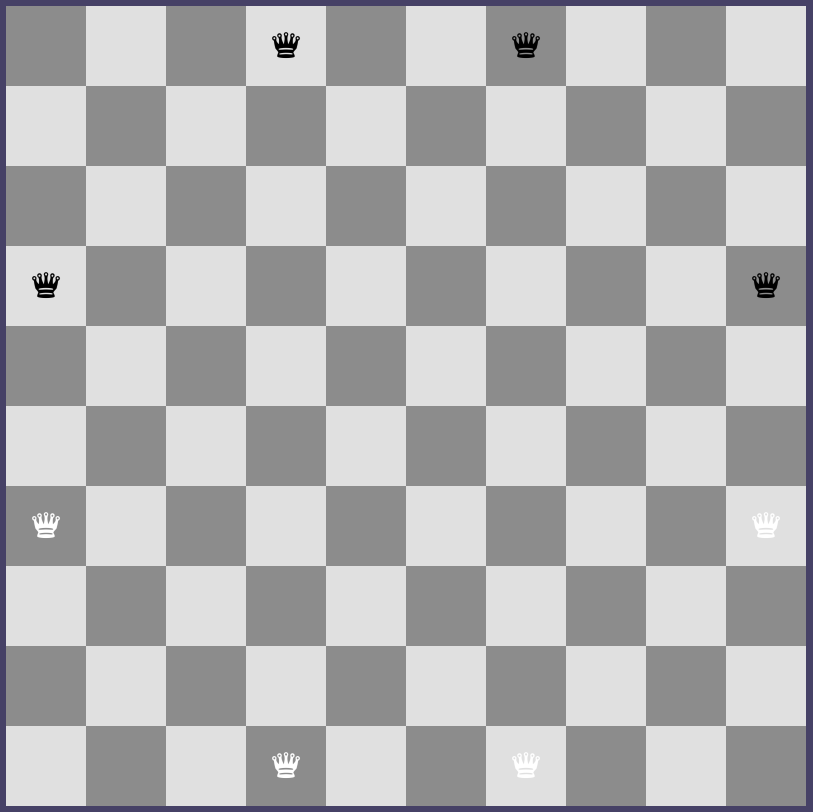
\includegraphics[width=\linewidth]{base_game_board_better.png}
        \caption{Position initiale}
        \label{fig:board_initial}
    \end{subfigure}
    \hspace{1.5cm}%
    \begin{subfigure}[t]{0.25\linewidth}
        \centering
        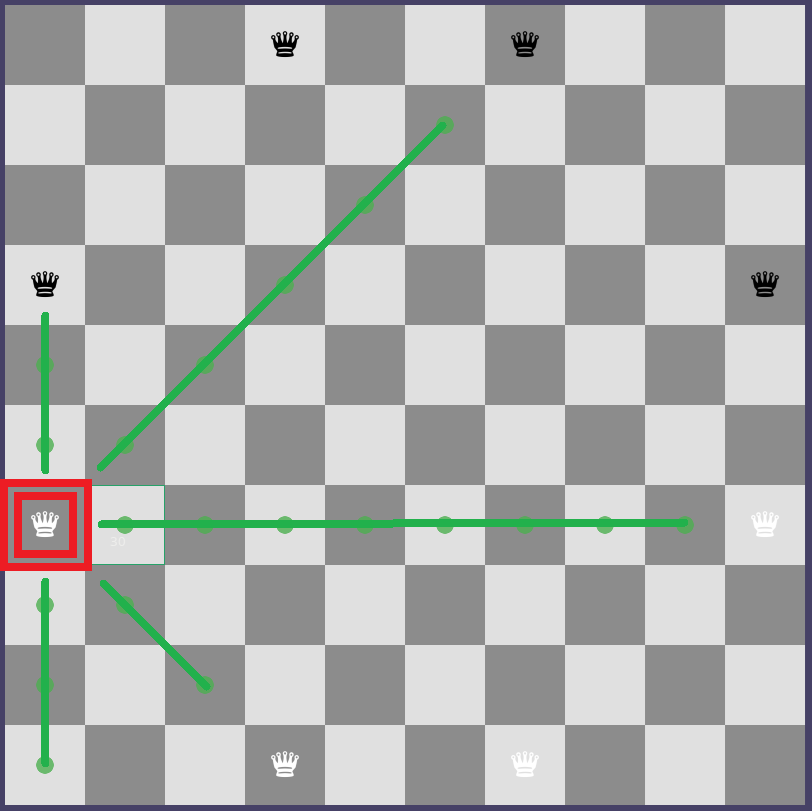
\includegraphics[width=\linewidth]{selecting_queen.png}
        \caption{Sélection de la reine : on sélectionne un nouvel emplacement pour la reine}
        \label{fig:board_select}
    \end{subfigure}
    
    \vspace{0.5cm}
    
    % --- Deuxième ligne ---
    \begin{subfigure}[t]{0.25\linewidth}
        \centering
        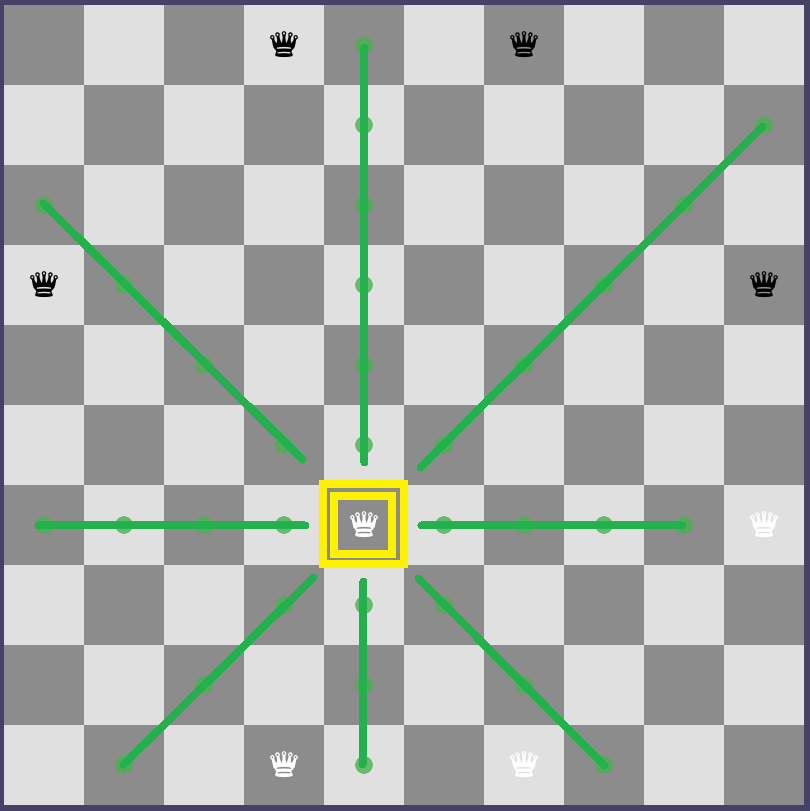
\includegraphics[width=\linewidth]{placing_arrow.png}
        \caption{Placement de la flèche : une fois la reine placée, on tire sur un nouvel endroit}
        \label{fig:board_place}
    \end{subfigure}
    \hspace{1.5cm}%
    \begin{subfigure}[t]{0.25\linewidth}
        \centering
        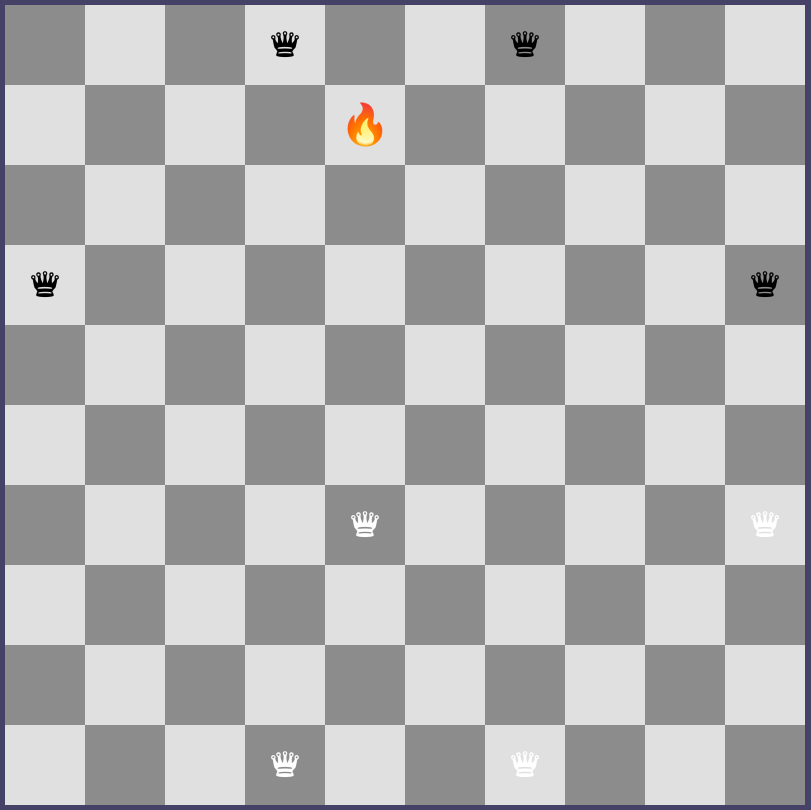
\includegraphics[width=\linewidth]{placed_arrow.png}
        \caption{Flèche placée}
        \label{fig:board_placed}
    \end{subfigure}

    \caption{Évolution d'une partie~: position initiale et premier coup}
    \label{fig:game_evolution}
\end{figure}

\subsection{Complexité} \label{sec:complexite}

Le jeu des Amazones est d'une très grande complexité~\cite{Hensgens2001}.
Le tableau ci-dessous emploie les abréviations Branch.~pour «~facteur de
branchement~» et Cmplx.~pour «~complexité~».

\begin{table}[H]
    \centering
\renewcommand{\arraystretch}{1.5}
\resizebox{\textwidth}{!}{
\begin{tabular}{ | p{4.5cm} || c | c | c | }
    \hline
    \textbf{} & \textbf{Échecs (8$\times$8)} & \textbf{Amazones (10$\times$10)} & \textbf{Go (19$\times$19)} \\
    \hline
    Facteur Branch. Initial
    & $\mathtt{\sim}$ 20
    & \makecell{$\mathtt{\sim}$ 2176}
    & $\mathtt{\sim}$ 361 \\
    \hline
    Facteur Branch. Moyen
    & $\mathtt{\sim}$ 35
    & \makecell{$\mathtt{\sim}$ 374 joueur de départ \\ $\mathtt{\sim}$ 299 deuxième joueur \\ $\mathtt{\sim}$50 durant la fin de partie}
    & $\mathtt{\sim}$ 250 \\
    \hline
    Nombre de tours moyen
    & $\mathtt{\sim}$ 80
    & $\mathtt{\sim}$ 84
    & $\mathtt{\sim}$ 150 \\
    \hline
    Cmplx. Arbre de jeu
    & $\mathtt{\sim} 10^{123}$
    & $\mathtt{\sim}$ 1.09 * $10^{212}$
    & $\mathtt{\sim} 10^{360}$ \\
    \hline
    Cmplx. Espaces d'états
    & \makecell{de $\mathtt{\sim}$ 3.7 * $10^{43}$ à $\mathtt{\sim}$ $10^{52}$}
    & $\mathtt{\sim}$ 6.45* $10^{40}$
    & $\mathtt{\sim}$ $10^{170}$ \\
    \hline
\end{tabular}
}
\caption{Comparaison des complexités pour des tailles de plateau traditionnelles (8$\times$8
pour les échecs, 10$\times$10 pour les Amazones, 19$\times$19 pour le Go)
\cite{Allis1994}\cite{Tromp2007}}
\end{table}
\renewcommand{\arraystretch}{1}

Comme l'illustre ce tableau comparatif, la complexité des Amazones réside
dans son facteur de branchement initial extrême, surpassant largement celui
des échecs et comparable à celui du Go. Bien que la profondeur de jeu soit
modérée, cette «~largeur~» excessive génère un arbre de jeu colossal
($10^{212}$), rendant toute exploration exhaustive impossible en raison de
l'explosion combinatoire. Pour contourner cette explosion, les approches
modernes s'appuient sur la sélectivité~: solveurs de preuve comme
\textit{df-pn}~\cite{Song2015Amazons}, algorithmes de jeu utilisant du
\textit{Forward Pruning}~\cite{Qian2015}, méthodes statistiques comme le MCTS
via l'Upper Confidence bounds applied to Trees (UCT)~\cite{Kocsis2006}, ou encore
le Machine Learning \cite{qian2026resource}.


\section{Algorithmes et structures de données}

\subsection{Moteur de jeu~: algorithmes}
\label{sec:engine-algo}

\subsubsection{Validation physique des déplacements (Algorithme de Raycasting)}

La règle principale des Amazones stipule qu'aucune pièce ne peut franchir
un obstacle. Pour valider mathématiquement un coup saisi par un joueur,
le moteur implémente un algorithme de vérification fonctionnant sur
le principe du lancer de rayon (\textit{Raycasting}) en grille discrète.

L'algorithme calcule d'abord le vecteur de déplacement $\vec{v} = (\Delta x, \Delta y)$
entre le point de départ $A(x_1, y_1)$ et le point d'arrivée $B(x_2, y_2)$,
puis vérifie que le mouvement respecte la contrainte de la dame aux échecs,
c'est-à-dire que $\Delta x = 0$, ou $\Delta y = 0$, ou $|\Delta x| = |\Delta y|$.
Il détermine ensuite un pas géométrique valant $-1$, $0$ ou $1$ pour chaque
axe, via la formule $step_x = \text{sign}(\Delta x)$ et
$step_y = \text{sign}(\Delta y)$. Une boucle itérative parcourt alors le
segment point par point~: si la carte globale des obstacles révèle une 
collision à la coordonnée courante, l'exploration s'interrompt prématurément et la trajectoire est déclarée invalide.

\subsubsection{Génération des coups possibles}
Le Jeu des Amazones se distingue par un facteur de branchement élevé. Contrairement aux échecs, une action n'est pas unitaire, mais séquentielle et interdépendante~: le déplacement d'une reine modifie immédiatement la topologie des obstacles pour le tir de la flèche qui suit. 

Pour fournir à l'intelligence artificielle l'ensemble exhaustif des coups légaux, le moteur implémente un algorithme de génération de l'arbre des possibles basé sur une exploration combinatoire contrainte. Cet algorithme opère en trois phases déterministes~:

Il isole le sous-ensemble $Q$ contenant les positions des quatre reines du joueur actif. Ensuite pour chaque reine $q \in Q$, l'algorithme effectue un balayage spatial omnidirectionnel pour déterminer $D_Q$, l'ensemble de ses cases de destination atteignables. Pour chaque destination candidate $d \in D_Q$, l'algorithme simule virtuellement le déplacement. Cette translation modifie l'état du plateau~: la case d'origine de la reine devient libre, et sa case d'arrivée devient un obstacle. Depuis cette nouvelle position $d$, une seconde expansion spatiale est calculée pour obtenir $D_A$, l'ensemble des cibles valides pour la flèche.

Le nombre total de coups possibles à un instant donné se calcule en additionnant toutes ces combinaisons. Cela se modélise par la formule mathématique suivante~:

$$ \text{Total des coups} = \sum_{q \in Q} \sum_{d \in D_Q} |D_A(d)| $$

Afin d'expliquer ce calcul plus simplement~:
    $Q$ représente le groupe des quatre reines du joueur actif.
    Pour chaque reine $q$, l'ensemble $D_Q$ désigne toutes les cases de destination qui lui sont accessibles.
    Pour chaque destination $d$ choisie, la notation $|D_A(d)|$ représente simplement le nombre exact de flèches qu'il est possible de tirer depuis cette nouvelle case.

Cette double somme illustre bien la mécanique «~à deux temps~» propre au jeu des Amazones. Aux échecs, le déplacement d'une pièce (comme un fou ou une tour) demande un calcul simple avec une complexité linéaire $\mathcal{O}(R)$, où $R$ est la distance maximale de déplacement. Dans notre moteur, le fait de lier le mouvement et le tir nous oblige à multiplier ces possibilités entre elles, élevant la complexité d'exploration à $\mathcal{O}(R^2)$ par pièce. C'est précisément pour supporter ce très grand volume de calculs que l'utilisation des structures \textit{Bitboards} s'est imposée pour l'Intelligence Artificielle.

\subsection{Le cœur du jeu et l'Intelligence Artificielle}
\label{sec:ai-alg-struct}

\subsubsection{Représentation de l'état et Complexité~: les Bitboards}

Pour garantir des performances optimales, nous avons modélisé le plateau
via des \textit{Bitboards} \cite{Browne2014}. Le plateau pouvant atteindre une taille de
$11 \times 11$ (121 cases), une simple variable de 64 bits était insuffisante.
Nous avons donc conçu une structure \texttt{Bitboard} composée de deux
entiers non signés ($2 \times$ \texttt{uint64\_t}), offrant 128 bits
d'espace. 

Cette architecture matérielle permet d'exécuter la majorité des opérations classiques
en temps constant $\mathcal{O}(1)$, comme les manipulations de masques (ET, OU, XOR) 
ainsi que les décalages de bits. Le calcul du 
débordement entre nos deux entiers 64 bits (\texttt{low} et \texttt{high}) ajoute un surcoût 
mineur, mais la complexité temporelle globale reste strictement bornée et indépendante de l'état du plateau.

La véritable puissance de cette structure, par rapport aux approches matricielles classiques,
s'exprime lors de la génération des trajectoires (\textit{slides}), qui s'effectue en temps constant
global $\mathcal{O}(1)$. Dans nos heuristiques, nous distinguons deux types de déplacements~:

\begin{itemize}
    \item Le \textbf{\textit{King step}}~: il simule une avancée d'une seule case dans les huit directions, pour savoir par exemple si une reine peut bouger. Il se calcule par de simples décalages de bits immédiats.
    \item Le \textbf{\textit{Queen slide}}~: il calcule la portée maximale d'une pièce avant de rencontrer un obstacle (le bord du plateau ou une autre pièce).
\end{itemize}

De manière naïve, calculer un \textit{Queen slide} nécessite des boucles itératives
conditionnelles (avancer d'une case, vérifier si elle est vide, continuer, sinon arrêter). Ces
boucles sont extrêmement coûteuses en temps d'exécution pour le processeur (étant appelées à chaque évaluation).

\paragraph{La solution~: l'algorithme de Kogge-Stone.}
Pour éliminer totalement ces boucles, nous avons implémenté l'algorithme de Kogge-Stone \cite{CPW_KoggeStone}.
Issu de l'architecture matérielle des additionneurs, cet algorithme repose sur le principe de propagation
parallèle (\textit{Parallel Prefix}). Au lieu d'avancer case par case, le processeur «~pousse~»
simultanément l'ensemble des pièces d'une même couleur à travers un masque représentant
les cases vides de la grille.

\paragraph{Mécanique des décalages exponentiels.}
Cette propagation s'effectue via une séquence stricte de quatre décalages bit-à-bit 
exponentiels. À chaque étape, la zone d'influence de la pièce double sa portée en s'appuyant 
sur le résultat de l'étape précédente.
Pour illustrer ce concept, prenons une ligne de 8 cases lue de gauche à droite. L'amazone part de la première case, et un obstacle (une flèche ou une autre pièce) occupe la sixième case~:
\begin{itemize}
    \item \textbf{État initial~:} 
    \newline \texttt{G = 1000 0000} (La pièce est sur le bit de poids fort)
    \newline \texttt{P = 0111 1\textbf{0}11} (Les cases vides : le premier '0' est la reine, le deuxième un mur)

    \item \textbf{Décalage de 1~:} La pièce s'étend sur 1 case adjacente vide. Le masque se décale lui aussi pour repérer les futurs blocs de 2 cases vides consécutives. (Il projete une "ombre" de taille équivalente au prochain décalage, pour ne pas pouvoir sauter par dessus cet obstacle)
    \newline \texttt{G = 1100 0000} (La portée est maintenant de 2 cases)
    \newline \texttt{P = 0011 1\textbf{00}1} (Mise à jour via un ET logique avec lui-même décalé de 1)

    \item \textbf{Décalage de 2~:} La pièce bondit de 2 cases d'un coup en s'appuyant sur le nouveau masque. Le masque repère les blocs de 4 cases vides.
    \newline \texttt{G = 1111 0000} (La portée continue de s'étendre)
    \newline \texttt{P = 0000 1\textbf{000}} (Plus qu'un seul emplacement valide pour un futur grand bond)

    \item \textbf{Décalage de 4~:} La pièce tente un bond de 4 cases, mais elle est bloquée par la raréfaction des '1' dans le masque.
    \newline \texttt{G = 1111 1000} (L'expansion s'arrête exactement \textit{devant} l'obstacle)
    \newline \texttt{P = 0000 0\textbf{000}} (Le masque se vide totalement)
    
    \item \textbf{Décalage de 8~:} Ultime étape pour les plateaux étendus, permettant de couvrir jusqu'à 15 cases (sans effet ici puisque \texttt{P} ne contient plus que des zéros).
\end{itemize}

Puisque la distance maximale franchissable sur notre plateau est de 10 cases (sur une grille $11 \times 11$), 
cette séquence couvre l'intégralité des trajectoires possibles. Ainsi, ce qui nécessiterait des dizaines
d'itérations conditionnelles dans une matrice classique est ici résolu de manière purement mathématique 
et simultanée en seulement quatre instructions.

Enfin, la seule complexité variable de notre modèle intervient lors de l'extraction des 
coups ou de l'évaluation des heuristiques. Bien que l'instruction matérielle d'extraction 
(\textit{Pop Least-Significant-Bit} ou \texttt{pop\_lsb}) s'exécute instantanément en $\mathcal{O}(1)$, 
elle est invoquée au sein d'une boucle pour lister les éléments actifs. Cette boucle s'exécutant 
exactement $k$ fois (où $k$ est le nombre strict de pièces ou cases évaluées), nous garantissons une 
complexité d'itération en $\mathcal{O}(k)$. Ce comportement est infiniment plus performant qu'un 
parcours complet de la grille en $\mathcal{O}(N)$ inhérent aux tableaux bidimensionnels.

\subsubsection{L'approche Minimax et ses heuristiques}

Le premier moteur d'IA repose sur l'algorithme Minimax, optimisé par
l'élagage Alpha-Beta \cite{GeeksforGeeks2026_AlphaBeta}. Pour pallier l'explosion combinatoire, nous avons
enrichi cette base par deux mécanismes paramétrables. L'approfondissement
itératif (\textit{Iterative Deepening}) garantit le renvoi du meilleur coup
trouvé à la profondeur maximale complétée si la limite de temps est atteinte.
L'élagage anticipé (\textit{Forward Pruning} \cite{Qian2015}) restreint la largeur du
faisceau de recherche en ne conservant que les coups offrant le plus de
contrôle de plateau. Sans ces optimisations, le système bascule de manière transparente
sur un Alpha-Beta exhaustif classique.

L'évaluation des nœuds feuilles constitue le cœur décisionnel de notre
stratégie. Nous avons conçu et comparé trois fonctions d'évaluation offrant
un compromis graduel entre rapidité et finesse mathématique.

La première approche est l'évaluation de mobilité \cite{Hensgens2001}, axée sur la mobilité relative (\texttt{eval\_me}),
calcule rapidement la différence entre le nombre total de coups légaux
disponibles pour les Blancs et les Noirs. En simulant une expansion de type
\textit{Queen slide} pour toutes les reines, l'algorithme dénombre les cases
uniques atteignables. Soit $M_p$ l'ensemble des cases atteignables par le
joueur $p$, l'heuristique est définie par~:
$$ \mathcal{H}_{me} = |M_{blanc}| - |M_{noir}| $$
Cette légèreté calculatoire permet d'atteindre d'excellentes profondeurs
d'exploration, mais l'évaluation demeure myope et peine à anticiper la
fermeture structurelle des territoires.

La deuxième heuristique, dite de territoire relatif (\texttt{eval\_rth}) \cite{Hensgens2001},
évalue le contrôle spatial en déployant un parcours en largeur (BFS)
simultané. Elle calcule la distance, en nombre de mouvements de Reine,
séparant chaque case vide de la pièce la plus proche. Soit $\mathcal{E}$
l'ensemble des cases vides, et $d_W(x)$ (resp. $d_B(x)$) la distance minimale
entre une case $x$ et une reine blanche (resp. noire)~:
$$ \mathcal{H}_{rth} = \sum_{x \in \mathcal{E}} \Delta(x) \quad \text{avec} \quad \Delta(x) =
\begin{cases}
\min(d_B(x), C) - d_W(x) & \text{si } d_W(x) < d_B(x) \\
-(\min(d_W(x), C) - d_B(x)) & \text{si } d_B(x) < d_W(x) \\
0 & \text{sinon}
\end{cases} $$
Une distance infinie est plafonnée par une constante $C$ (définie par
$C = \text{taille du plateau} + 2$).

Notre modèle le plus abouti repose sur les territoires absolus combinés
(\texttt{eval\_qdkd}) \cite{Lieberum2005}. Il simule l'appropriation du plateau par une
expansion continue (\textit{flood-fill}) traitée case par case. La force
de cette heuristique réside dans sa résolution des conflits~: si une case
est atteinte par les deux joueurs à la même itération $k$, elle est déclarée
contestée et agit comme un obstacle infranchissable. Soient $T_Q(p)$ et
$T_K(p)$ les ensembles de cases conquises par le joueur $p$ selon des
déplacements respectifs de Reine et de Roi~:
$$ t_1 = |T_Q(Blanc)| - |T_Q(Noir)| \qquad t_2 = |T_K(Blanc)| - |T_K(Noir)| $$
Le calcul final applique une pondération mariant vision globale et contrôle
local~ (choisi d'après les pistes de calcul de Lieberum \cite{Lieberum2005}) :
$$ \mathcal{H}_{qdkd} = 1.0 \times t_1 + 0.5 \times t_2 $$

\subsubsection{Monte Carlo Tree Search (MCTS) et apprentissage automatique}

Le second moteur d'IA exploite le Monte Carlo Tree Search. Pour modéliser
l'arborescence, nous avons opté pour une structure de données
\textbf{LCRS} (\textit{Left-Child Right-Sibling}) \cite{GeeksforGeeks2025_LCRS}. Ce choix découle
directement du facteur de branchement initial supérieur à 2\,000 coups
possibles~: utiliser des tableaux de pointeurs pour stocker les enfants
de chaque nœud aurait provoqué une explosion de l'empreinte mémoire.
Le choix de la structure LCRS (\textit{Left-Child Right-Sibling}) répond à une contrainte majeure du jeu des Amazones~: son facteur de branchement exceptionnellement élevé (entre 500 et 2\,000 coups possibles par tour). Une approche classique, où chaque nœud pré-allouerait un tableau pointant vers tous ses enfants potentiels, saturerait la mémoire système de manière quasi instantanée. 

À l'inverse, l'approche LCRS garantit une empreinte mémoire minimale et fixe. Chaque nœud ne contient que deux pointeurs~: l'un vers son premier enfant, l'autre vers son frère immédiat. Cette optimisation spatiale implique un compromis temporel, car l'accès au $k$-ième enfant nécessite un parcours séquentiel en $O(k)$ cycles CPU. 

Cependant, ce coût est largement justifié. Couplée à une instanciation dynamique des enfants --- où un nœud n'est créé que lorsque le coup correspondant est réellement exploré --- cette architecture empêche l'explosion mémoire tout en garantissant l'efficacité du moteur.
Nous avons également enrichi ce MCTS d'un réseau de neurones. Dans ce mode,
l'évaluation des nœuds non terminaux est combinée à l'inférence d'un modèle 
TensorFlow recevant en entrée un tenseur à quatre canaux généré par nos bitboards.

\paragraph{Politique de sélection UCT standard.}
Dans sa version classique, le MCTS guide la phase de sélection de l'arborescence à l'aide de la formule \textbf{UCT} (\textit{Upper Confidence bounds applied to Trees}) \cite{Kocsis2006}. Cette métrique applique les principes des bandits manchots à la recherche arborescente afin de trouver le compromis mathématique optimal entre l'exploitation des branches prometteuses et l'exploration des chemins peu visités. Pour un nœud enfant $n$, l'évaluation s'écrit~:

$$ \text{UCT}(n) = Q(n) + c \cdot \sqrt{\frac{\ln(N(parent))}{N(n)}} $$

où $Q(n)$ représente la valeur moyenne empirique du nœud (le taux de victoire obtenu par les simulations aléatoires), $N(parent)$ et $N(n)$ désignent respectivement le nombre total de visites du nœud parent et de l'enfant évalué, et $c$ est la constante d'exploration (théoriquement fixée à $\sqrt{2}$). Le premier terme favorise l'exploitation pure, tandis que le second garantit une exploration continue~: la racine carrée croît de manière logarithmique avec les visites du parent, forçant l'algorithme à évaluer les enfants délaissés (où $N(n)$ est faible ou nul).

\paragraph{Variante PUCT pour l'apprentissage automatique.} 
Lorsque le réseau de neurones est activé, la politique de sélection UCT classique est remplacée par la variante \textbf{PUCT} (\textit{Predictor + Upper Confidence Bound}) \cite{Cazenave2022}. Cette approche hybride combine l'exploration statistique d'UCT avec une évaluation par réseau de neurones pour guider plus efficacement la recherche.

La formule PUCT pour un nœud enfant $n$ s'écrit~:
$$ \text{PUCT}(n) = \frac{Q_{\text{rollout}}(n) + Q_{\text{NN}}(n)}{2} + c_{\text{puct}} \cdot \frac{\sqrt{N(parent)}}{1 + N(n)} $$

où $Q_{\text{rollout}}(n)$ est le taux de victoire empirique obtenu par les simulations Monte Carlo, $Q_{\text{NN}}(n)$ est la probabilité de victoire prédite par le réseau de neurones, $N(parent)$ et $N(n)$ sont respectivement les nombres de visites du parent et de l'enfant, et $c_{\text{puct}}$ est une constante d'exploration (par défaut 1.5).

Le réseau de neurones utilisé est un modèle de régression linéaire simple entraîné sur des parties auto-générées. Il reçoit en entrée un tenseur de dimension $11 \times 11 \times 4$ représentant~:
\begin{itemize}
    \item Canal 0~: positions des reines blanches (1 si présente, 0 sinon)
    \item Canal 1~: positions des reines noires
    \item Canal 2~: positions des flèches
    \item Canal 3~: masque de validité du plateau (1 pour les cases valides)
\end{itemize}

Cette architecture à quatre canaux permet au modèle de capturer simultanément la configuration matérielle et la topologie du plateau. Lors de la sélection, si l'évaluation neuronale d'un nœud n'a pas encore été calculée (\texttt{ai\_eval} $\leq -2.0$), le tenseur correspondant est généré à la volée et soumis au modèle TensorFlow. La valeur retournée est ensuite mise en cache dans le nœud pour éviter les inférences redondantes.


 
%------------------------------------------------------------------------------
% SECTION 2.2 - Structures de données et protocole réseau
%------------------------------------------------------------------------------
 
\subsection{Réseau~: structures de données et protocole}
\label{sec:network-data}
 
La mise en place du mode multijoueur a nécessité de résoudre deux contraintes
fondamentales de la programmation réseau~: la nature orientée flux du protocole
TCP et la nécessité de maintenir un état cohérent pour chaque connexion
asynchrone.
 
\subsubsection{Le problème du \textit{Framing} TCP}
\label{subsec:tcp-framing}
 
Contrairement à UDP qui fonctionne par datagrammes délimités, TCP est orienté
flux~: l'émetteur peut envoyer trois messages de 100 octets, mais le récepteur
pourrait recevoir un bloc de 250 octets suivi d'un fragment de 50 octets. Ce
phénomène, appelé \textit{TCP Framing}, rend impossible la lecture directe de
messages individuels sans mécanisme de délimitation.
 

Nous avons donc opté pour un délimiteur de fin de message (\texttt{'\textbackslash{}n'})
plutôt qu'un préfixe de longueur. Ce choix présente deux avantages~:
il permet le débogage à l'œil nu via des outils standards (\texttt{netcat},
\texttt{tcpdump}), et il évite les problèmes de désynchronisation si un octet est corrompu, une erreur dont la récupération serait impossible
sans fermer la connexion.
 
\paragraph{}
Pour accumuler les fragments TCP jusqu'à réception d'un message complet, chaque
connexion dispose de son propre tampon linéaire de 4\,096 octets. Ce
dimensionnement (environ 2,7 fois le MTU Ethernet standard de 1\,500 octets)
garantit qu'au moins deux messages complets peuvent être mis en file
simultanément, absorbant ainsi les pics de trafic sans saturation.
 
\paragraph{}
L'extraction des messages s'effectue en trois phases distinctes. L'\textbf{accumulation}~  consiste en la concaténation à la fin du tampon des octets bruts reçus via
\texttt{recv()}. Ensuite avec la
\textbf{recherche}~ linéaire on localise le premier caractère
de fin de ligne dans le tampon. Enfin
le message extrait est \textbf{copié} vers un tampon de sortie, puis les octets restants
sont décalés vers le début du tampon via \texttt{memmove()}, préservant ainsi
les fragments du message suivant. Cette dernière opération, bien que coûteuse
en temps ($\mathcal{O}(n)$ où $n$ est la taille des données restantes), reste
négligeable face aux latences réseau et garantit une gestion mémoire sans
fragmentation.



\begin{center}
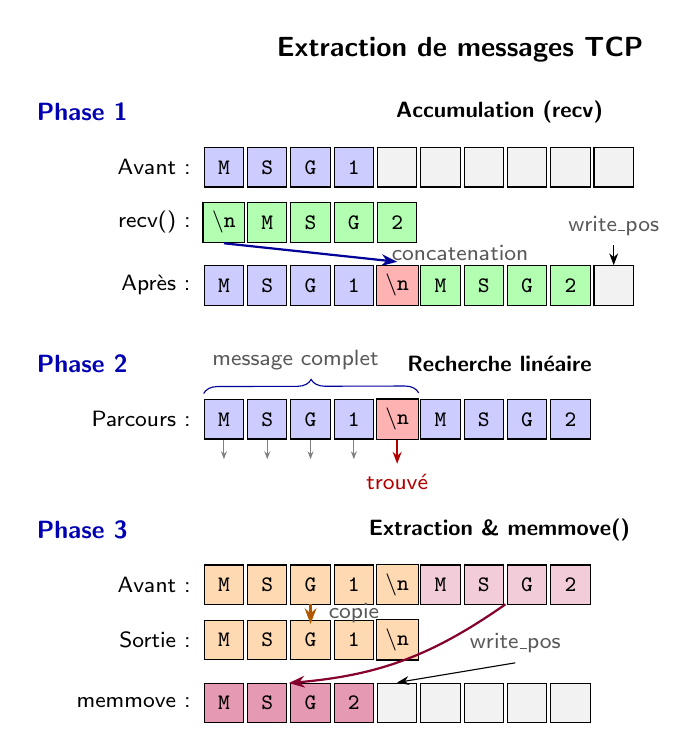
\begin{tikzpicture}[
    cell/.style={draw, minimum width=0.5cm, minimum height=0.5cm, font=\ttfamily\footnotesize},
    datacell/.style={cell, fill=blue!20},
    newdatacell/.style={cell, fill=green!30},
    newlinecell/.style={cell, fill=red!30},
    emptycell/.style={cell, fill=gray!10},
    extractedcell/.style={cell, fill=orange!30},
    remaincell/.style={cell, fill=purple!20},
    movedcell/.style={cell, fill=purple!40},
    label/.style={font=\sffamily\footnotesize},
    phase/.style={font=\sffamily\bfseries\small, text=blue!70!black},
    arrow/.style={-{Stealth[length=2mm]}, thick, draw=blue!60!black},
    brace/.style={decorate, decoration={brace, amplitude=5pt, raise=2pt}},
    annotation/.style={font=\sffamily\footnotesize, text=gray!70!black},
]

% Titre
\node[font=\sffamily\bfseries, text=black] at (3, 0.8) {Extraction de messages TCP};

% ============================================================
% PHASE 1 : ACCUMULATION
% ============================================================
\node[phase] at (-1.8, 0) {Phase 1};
\node[font=\sffamily\bfseries\footnotesize] at (3.5, 0) {Accumulation (recv)};

% Tampon avant recv
\node[label, anchor=east] at (-0.3, -0.7) {Avant :};
\foreach \i/\c in {0/M, 1/S, 2/G, 3/1} {
    \node[datacell] (before\i) at (\i*0.55, -0.7) {\c};
}
\foreach \i in {4,5,6,7,8,9} {
    \node[emptycell] (before\i) at (\i*0.55, -0.7) {};
}

% Données reçues
\node[label, anchor=east] at (-0.3, -1.4) {recv() :};
\foreach \i/\c in {0/\textbackslash n, 1/M, 2/S, 3/G, 4/2} {
    \node[newdatacell] (recv\i) at (\i*0.55, -1.4) {\c};
}

% Flèche de concaténation
\draw[arrow] (recv0.south) to node[right, annotation, xshift=9mm] {concatenation} (2.2, -1.9);

% Tampon après recv
\node[label, anchor=east] at (-0.3, -2.2) {Après :};
\foreach \i/\c in {0/M, 1/S, 2/G, 3/1} {
    \node[datacell] (after\i) at (\i*0.55, -2.2) {\c};
}
\node[newlinecell] (after4) at (4*0.55, -2.2) {\textbackslash n};
\foreach \i/\c in {5/M, 6/S, 7/G, 8/2} {
    \node[newdatacell] (after\i) at (\i*0.55, -2.2) {\c};
}
\node[emptycell] (after9) at (9*0.55, -2.2) {};

\draw[{Stealth[length=1.5mm]}-] (after9.north) -- ++(0, 0.25) node[above, annotation] {write\_pos};

% ============================================================
% PHASE 2 : RECHERCHE LINÉAIRE
% ============================================================
\node[phase] at (-1.8, -3.2) {Phase 2};
\node[font=\sffamily\bfseries\footnotesize] at (3.5, -3.2) {Recherche linéaire};

% Tampon avec recherche
\node[label, anchor=east] at (-0.3, -3.9) {Parcours :};
\foreach \i/\c in {0/M, 1/S, 2/G, 3/1} {
    \node[datacell] (search\i) at (\i*0.55, -3.9) {\c};
}
\node[newlinecell] (search4) at (4*0.55, -3.9) {\textbackslash n};
\foreach \i/\c in {5/M, 6/S, 7/G, 8/2} {
    \node[datacell] (search\i) at (\i*0.55, -3.9) {\c};
}

% Flèches de parcours
\foreach \i in {0,1,2,3} {
    \draw[-{Stealth[length=1mm]}, gray] (search\i.south) -- ++(0, -0.25);
}
\draw[-{Stealth[length=1.5mm]}, red!70!black, thick] (search4.south) -- ++(0, -0.3) node[below, font=\sffamily\footnotesize, text=red!70!black] {trouvé};

% Accolade pour message complet
\draw[brace, blue!60!black] (search0.north west) -- (search4.north east) 
    node[midway, above=7pt, annotation, xshift=-2mm] {message complet};

% ============================================================
% PHASE 3 : EXTRACTION ET DÉCALAGE
% ============================================================
\node[phase] at (-1.8, -5.3) {Phase 3};
\node[font=\sffamily\bfseries\footnotesize] at (3.5, -5.3) {Extraction \& memmove()};

% Tampon source
\node[label, anchor=east] at (-0.3, -6) {Avant :};
\foreach \i/\c in {0/M, 1/S, 2/G, 3/1} {
    \node[extractedcell] (ext\i) at (\i*0.55, -6) {\c};
}
\node[extractedcell] (ext4) at (4*0.55, -6) {\textbackslash n};
\foreach \i/\c in {5/M, 6/S, 7/G, 8/2} {
    \node[remaincell] (ext\i) at (\i*0.55, -6) {\c};
}

% Tampon de sortie
\node[label, anchor=east] at (-0.3, -6.7) {Sortie :};
\foreach \i/\c in {0/M, 1/S, 2/G, 3/1} {
    \node[extractedcell] (out\i) at (\i*0.55, -6.7) {\c};
}
\node[extractedcell] (out4) at (4*0.55, -6.7) {\textbackslash n};

% Flèche copie
\draw[arrow, orange!70!black] (2*0.55, -6.25) -- (2*0.55, -6.5) node[midway, right, annotation, xshift=1mm, yshift=0.2mm] {copie};

% Tampon après memmove
\node[label, anchor=east] at (-0.3, -7.5) {memmove :};
\foreach \i/\c in {0/M, 1/S, 2/G, 3/2} {
    \node[movedcell] (moved\i) at (\i*0.55, -7.5) {\c};
}
\foreach \i in {4,5,6,7,8} {
    \node[emptycell] (moved\i) at (\i*0.55, -7.5) {};
}

% Flèche memmove
\draw[arrow, purple!70!black, bend left=15] (6.5*0.55, -6.25) to node[right, annotation, xshift=4mm] {} (1.5*0.55, -7.25);

% Nouveau write_pos
\draw[{Stealth[length=1.5mm]}-] (moved4.north) -- ++(1.5, 0.25) node[above, annotation] {write\_pos};

\end{tikzpicture}
\end{center}
 
\subsubsection{Protocole applicatif et sérialisation}
\label{subsec:protocol}
 
Au-dessus de la couche de framing, nous avons défini un protocole applicatif
textuel structuré autour d'une unité atomique~: le \texttt{Packet}.
 
\paragraph{}
Le format ASCII a été préféré au binaire pour trois raisons. Premièrement, il
élimine les problèmes de l'ordre dans lequel les octets sont placés lors de la communication
entre architectures hétérogènes (x86, ARM). Deuxièmement, il facilite le
débogage sans outils spécialisés~: un simple \texttt{netcat} suffit à observer
les échanges. Troisièmement, il permet une évolution du protocole par ajout de
nouveaux types de messages sans rétrocompatibilité binaire complexe.
 
\paragraph{}
Chaque paquet suit le format \texttt{"TYPE|PAYLOAD\textbackslash{}n"}, où
\texttt{TYPE} est un entier identifiant le type de message, le caractère
\texttt{'|'} sert de séparateur unique entre le type et la charge utile, et
le caractère \texttt{'\textbackslash{}n'} permet à la couche de framing de
détecter la fin du message. Cette conception garantit un parsing déterministe
en $\mathcal{O}(m)$ où $m$ est la longueur du message.
 
Le protocole définit 27 types de paquets répartis en trois catégories~: les
messages client vers serveur (préfixés \texttt{C2S\_}), les messages serveur
vers client (préfixés \texttt{S2C\_}), et les messages bidirectionnels. Le
tableau~\ref{tab:protocol-types} en annexe présente l'ensemble des types avec
leur rôle respectif.
 
\newpage
\subsection{Moteur de jeu~: structures de données}
\label{sec:engine-data}

Afin de garantir un moteur de jeu rapide et évolutif tout en anticipant
les besoins de calcul intensif de l'intelligence artificielle, une attention
particulière a été portée à la conception des structures de données de bas
niveau.

\subsubsection{Modélisation matricielle de l'état du jeu}

L'état global de la partie est encapsulé dans une structure unique
\texttt{GameState}. La représentation structurelle de base du plateau est
stockée sous forme d'un tableau dynamique à deux dimensions (matrice de type
\texttt{CellContent** board}). Chaque cellule contient une énumération
définissant son état (\texttt{CONTENT\_EMPTY}, \texttt{CONTENT\_WHITE\_QUEEN},
\texttt{CONTENT\_ARROW}, etc.). Cette modélisation matricielle offre une
lisibilité optimale pour l'affichage et permet un accès spatial en temps
constant $\mathcal{O}(1)$. Cependant, elle montre de fortes limites pour
l'exploration de l'arbre par l'IA~: le parcours itératif d'une matrice 2D
deviendrait un goulot d'étranglement lors des millions de simulations
nécessaires, d'où le recours aux bitboards décrits plus haut.

\subsubsection{Architecture Bitboard}

Le moteur maintient et consolide l'état du jeu à travers trois
\texttt{Bitboards} distincts, extraits dynamiquement depuis le
\texttt{GameState}~: \texttt{bb\_white} pour la position des reines blanches,
\texttt{bb\_black} pour les reines noires, et \texttt{bb\_arrows} pour
l'ensemble des flèches tirées. Cette représentation secondaire parallèle est
indispensable pour l'IA et les fonctions d'évaluation, tandis que la
représentation matricielle reste utilisée pour l'affichage et la validation
unitaire des règles.

\subsection{Interface graphique~: structures de données}
\label{sec:gui-data}

L'interface graphique s'appuie sur la boîte à outils GTK4~\cite{gtk4doc},
qui suit un paradigme orienté objet.

\subsubsection{Le contexte applicatif \texttt{GuiContext}}

De façon symétrique à l'architecture de la couche terminal, toute
l'information d'état de l'interface graphique est regroupée dans un objet global
\texttt{GuiContext}. Ce patron d'encapsulation (\textit{Context Object}) évite les variables
globales et facilite le passage d'état entre les différents gestionnaires
d'événements. 

Cette structure centralise tous les sous-systèmes~: la configuration du jeu, l'état courant de la partie (\texttt{GameState}), le conteneur principal de la fenêtre, mais également le moteur d'IA et le gestionnaire réseau (\texttt{NetworkManager}). Le regroupement de ces instances permet au contrôleur graphique d'orchestrer des parties locales, contre l'IA, ou en multijoueur réseau de façon transparente.

Le plateau de jeu visuel est représenté par un tableau unidimensionnel de conteneurs
de taille $n \times n$. Ce choix d'aplatissement (indexé par \texttt{y * size + x}) simplifie les calculs de conversion de coordonnées matricielles et évite la fragmentation en mémoire.

\subsubsection{L'automate des phases de jeu}

Un tour aux Amazones est indivisible~: déplacer une reine puis tirer une
flèche constitue une seule action logique. Pour modéliser cette contrainte
dans l'interface graphique, nous avons défini une machine à états finis régie par
deux statuts~: \texttt{PHASE\_MOVE\_QUEEN} et \texttt{PHASE\_SHOOT\_ARROW}. Ce mécanisme
garantit que l'interface est un automate déterministe~: un événement de clic ou de
glisser-déposer n'est traité que si l'état courant correspond à l'action
attendue par les règles du jeu.

\subsubsection{Les raccourcis clavier \texttt{KeyBindings}}

Une structure \texttt{KeyBindings} stocke sous forme de chaînes de caractères
(au format d'accélérateurs logiciels, ex: \texttt{"<Control>n"}) les
raccourcis clavier de l'application, modifiables en direct. À chaque modification,
le contrôleur de raccourcis de la fenêtre est dynamiquement détruit puis recréé,
garantissant une cohérence stricte entre la vue des paramètres et le déclenchement
des actions.

\newpage

%==============================================================================
\section{Architecture du projet}
\label{sec:architecture}
%==============================================================================

\subsection{Découpage en modules}

L'application suit une architecture en couches respectant strictement le principe de séparation des responsabilités. La figure~\ref{fig:arch-layers} illustre les dépendances entre modules.

\begin{figure}[H]
\centering
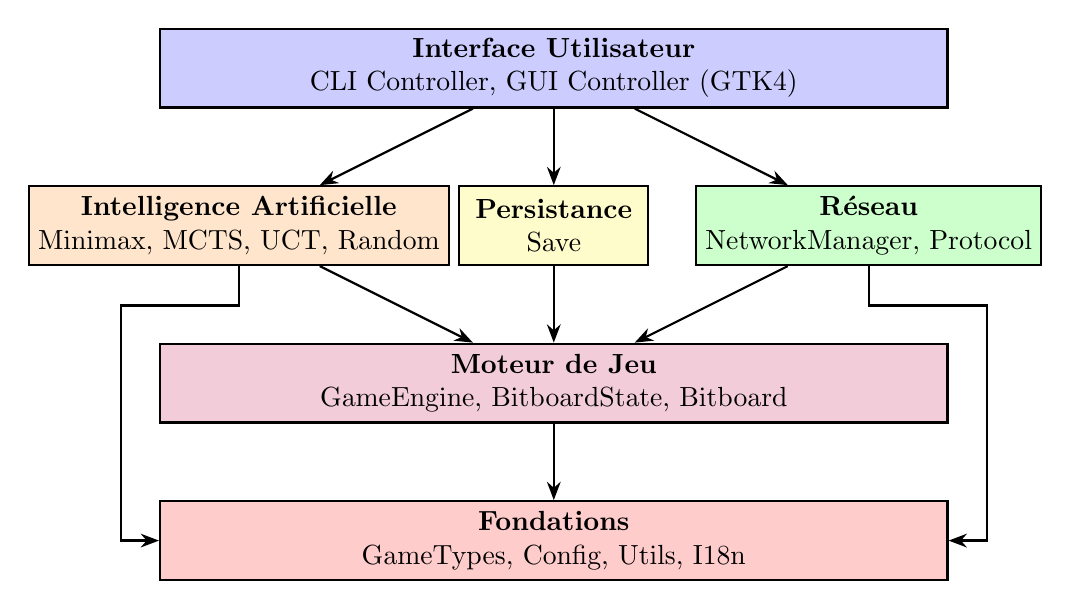
\begin{tikzpicture}[
    layer/.style={rectangle, draw, thick, minimum height=1cm, align=center},
    arrow/.style={->, >=Stealth, thick}
]
% Layers
\node[layer, fill=blue!20, minimum width=10cm] (ui) at (0,2) {\textbf{Interface Utilisateur} \\ CLI Controller, GUI Controller (GTK4)};

\node[layer, fill=orange!20, minimum width=3.2cm] (ai) at (-4,0) {\textbf{Intelligence Artificielle} \\ Minimax, MCTS, UCT, Random};
\node[layer, fill=yellow!20, minimum width=2.4cm] (save) at (0,0) {\textbf{Persistance} \\ Save};
\node[layer, fill=green!20, minimum width=3.2cm] (net) at (4,0) {\textbf{Réseau} \\ NetworkManager, Protocol};

\node[layer, fill=purple!20, minimum width=10cm] (engine) at (0,-2) {\textbf{Moteur de Jeu} \\ GameEngine, BitboardState, Bitboard};

\node[layer, fill=red!20, minimum width=10cm] (core) at (0,-4) {\textbf{Fondations} \\ GameTypes, Config, Utils, I18n};

% Arrows from UI to middle layer
\draw[arrow] (ui) -- (ai);
\draw[arrow] (ui) -- (save);
\draw[arrow] (ui) -- (net);

% Arrows from middle layer to Engine
\draw[arrow] (ai) -- (engine);
\draw[arrow] (save) -- (engine);
\draw[arrow] (net) -- (engine);

% Arrow from Engine to Core
\draw[arrow] (engine) -- (core);

% Arrows from middle layer to Core (contournement extérieur)
\draw[arrow] (ai.south) -- ++(0,-0.5) -- ++(-1.5,0) |- (core.west);
\draw[arrow] (net.south) -- ++(0,-0.5) -- ++(1.5,0) |- (core.east);

\end{tikzpicture}
\caption{Architecture en couches du projet. Les flèches représentent les dépendances~: chaque module dépend uniquement des couches inférieures, garantissant testabilité et maintenabilité.}
\label{fig:arch-layers}
\end{figure}

Le moteur de jeu constitue le \textbf{noyau pur} de l'application~: totalement indépendant de l'affichage et du réseau, il expose une API pour la manipulation de l'état du jeu. Les modules d'IA interrogent ce moteur via l'interface \texttt{BitboardState} pour des calculs haute performance, tandis que les contrôleurs manipulent le \texttt{GameState}. Le réseau et l'IA communiquent avec l'interface via un système de \textbf{callbacks}, évitant ainsi toute dépendance cyclique.

\subsection{Résumé de l'architecture}

Le jeu des Amazones est organisé en trois couches distinctes.

\paragraph{Interface utilisateur}

Deux modes d'interaction sont disponibles via l'interface \texttt{Controller}. Le \texttt{CLI\_Controller} offre une interface en ligne de commande utilisant la bibliothèque \texttt{readline}, tandis que le \texttt{GUI\_Controller} propose une interface graphique basée sur GTK4. Ces deux contrôleurs partagent les mêmes dépendances vers les services de la couche inférieure.

\paragraph{Services}

La couche services regroupe la logique métier en trois modules. L'\texttt{AI\_Interface} constitue une interface polymorphe pour les algorithmes d'IA, définissant la méthode \texttt{get\_best\_move()}. Le \texttt{GameEngine} gère les règles du jeu, applique les coups et détecte la fin de partie. Enfin, le \texttt{NetworkManager} assure la gestion du multijoueur via TCP/IP avec découverte automatique des serveurs sur le réseau local.

\paragraph{Données}

La couche données contient les structures fondamentales du système. \texttt{GameState} encapsule l'état complet de la partie, incluant le plateau, le joueur actuel et les piles undo/redo. \texttt{Move} représente un coup complet avec la position source, la destination et la position de la flèche. \texttt{Bitboard} offre une représentation binaire compacte sur 128 bits permettant des calculs rapides, et \texttt{BitboardState} agrège trois bitboards distincts pour les reines blanches, les reines noires et les flèches.

\paragraph{Patrons de conception}

L'architecture exploite plusieurs patrons de conception classiques. Le patron \textit{Strategy} permet de substituer les algorithmes d'IA de manière transparente. Le patron \textit{Factory} délègue la création des IA à un module dédié. Le patron \textit{Observer} gère les événements réseau de manière asynchrone via des callbacks. Le patron \textit{Façade} simplifie l'accès au \texttt{GameEngine} en masquant la complexité des opérations sur les bitboards.

Cette architecture modulaire facilite les tests, la maintenance et l'évolution du projet.

% Diagramme UML de classes simplifié - Jeu des Amazones
% Nécessite: \usepackage{tikz}
%           \usetikzlibrary{positioning, arrows.meta, shapes.multipart, calc}

\begin{figure}[H]
\centering
\begin{tikzpicture}[
    node distance=2cm and 2.5cm,
    >=Stealth,
    % Classes avec 2 parties
    class/.style={
        rectangle split,
        rectangle split parts=2,
        rectangle split part fill={#1!25, white},
        draw=#1!70!black,
        thick,
        font=\small,
        align=center,
        minimum width=3cm
    },
    % Boîtes simples
    box/.style={
        rectangle,
        draw=#1!70!black,
        fill=#1!25,
        thick,
        font=\small,
        minimum width=2.4cm,
        minimum height=1cm
    },
    % Flèches UML
    inherit/.style={-{Triangle[open, length=2.5mm, width=2mm]}, thick},
    compo/.style={-{Diamond[length=2.5mm, width=2mm, fill=black]}, thick},
    depend/.style={->, thick, dashed},
    assoc/.style={->, thick}
]

% ============== COUCHE 1 : UI ==============

\node[class=blue] (Controller) at (0, 0) {
    \textbf{«interface» Controller}
    \nodepart{second}
    run\_mode()
};

\node[box=blue] (CLI) at (-3.5, -2.5) {\textbf{CLI\_Controller}};
\node[box=blue] (GUI) at (3.5, -2.5) {\textbf{GUI\_Controller}};

% Héritage Controllers
\draw[thick] (CLI.north) -- ++(0, 0.6) -| (0, -1.9);
\draw[thick] (GUI.north) -- ++(0, 0.6) -| (0, -1.9);
\draw[inherit] (0, -1.9) -- (Controller.south);

% ============== COUCHE 2 : SERVICES ==============

\node[class=orange] (AI) at (-6, -6) {
    \textbf{«interface» AI\_Interface}
    \nodepart{second}
    get\_best\_move()
};

\node[class=teal] (Engine) at (0, -6) {
    \textbf{«module» GameEngine}
    \nodepart{second}
    apply\_move()\\is\_game\_over()
};

\node[class=green!70!black] (Network) at (6, -6) {
    \textbf{NetworkManager}
    \nodepart{second}
    SendMove()
};

% Implémentations AI
\node[box=orange, minimum width=1.8cm] (Minimax) at (-7, -8.5) {\footnotesize Minimax};
\node[box=orange, minimum width=1.6cm] (MCTS) at (-5, -8.5) {\footnotesize MCTS};

% Héritage AI
\draw[thick] (Minimax.north) -- ++(0, 0.5) -| (-6, -8);
\draw[thick] (MCTS.north) -- ++(0, 0.5) -| (-6, -8);
\draw[inherit] (-6, -8) -- (AI.south);

% ============== COUCHE 3 : DONNÉES ==============

\node[class=cyan!80] (GameState) at (0, -10.5) {
    \textbf{GameState}
    \nodepart{second}
    board, player, status
};

\node[box=gray] (Move) at (-4.5, -13) {\textbf{Move}};

\node[class=violet] (Bitboard) at (5.5, -10.5) {
    \textbf{Bitboard}
    \nodepart{second}
    low, high
};

\node[class=violet] (BitboardState) at (5.5, -13.5) {
    \textbf{BitboardState}
    \nodepart{second}
    white, black, arrows
};

% ============== RELATIONS ==============

% CLI -> AI : passe à gauche de CLI, descend, arrive sur AI.north
\draw[depend] 
    (CLI.west) 
    -- ++(-1.5, 0) 
    -- ++(0, -2.5) 
    -- (AI.north);

% CLI -> Engine : descend de CLI, tourne, arrive sur Engine.north
\draw[depend] 
    ($(CLI.south) + (-0.3, 0)$) 
    -- ++(0, -0.8) 
    -| ($(Engine.north) + (-0.4, 0)$);

% GUI -> Engine : descend de GUI, tourne, arrive sur Engine.north
\draw[depend] 
    ($(GUI.south) + (0.3, 0)$) 
    -- ++(0, -0.8) 
    -| ($(Engine.north) + (0.4, 0)$);

% CLI -> Network : passe au-dessus, contourne GUI, arrive sur Network.north
\draw[depend] 
    (CLI.east) 
    -- ++(0.5, 0)
    -- ++(0, 0.8)
    -- ++(7, 0)
    -- ++(0, -3.3)
    -- (Network.north);

% GUI -> Network : passe à droite de GUI, arrive sur Network.north
\draw[depend] 
    (GUI.east) 
    -- ++(1.5, 0) 
    -- ++(0, -2.5) 
    -- ($(Network.north) + (0.4, 0)$);

% AI -> GameState : descend de AI, passe sous Minimax/MCTS, arrive sur GameState.west
\draw[depend] 
    ($(AI.south) + (-0.5, 0)$) 
    -- ++(0, -3.5) 
    -- ++(4, 0)
    -- (GameState.west);

\draw[depend] 
    (AI.east)
    -- ++(1, -3.5) 
    -- ++(7, 0)
    -- (BitboardState.west);

% Engine -> GameState : descend directement
\draw[assoc] 
    (Engine.south) 
    -- node[right, font=\scriptsize] {uses} 
    (GameState.north);



% Engine -> BitboardState : sort à droite (plus bas), descend plus, arrive sur BitboardState.west
\draw[depend] 
    ($(Engine.east) + (0, -0.3)$) 
    -- ++(1.5, 0)
    -- ++(0, -7)
    -- (BitboardState.west);

% GameState -> Move : composition, sort en bas à gauche, arrive sur Move.east
\draw[compo] 
    ($(GameState.south) + (-0.5, 0)$) 
    -- ++(0, -0.8)
    -- ++(-2.5, 0)
    -- (Move.east);

% Network -> Move : descend, passe sous tout, remonte vers Move.south
\draw[depend] 
    (Network.east) 
    -- ++(0, -6)
    -- ++(-9, 0)
    -- ++(0, -1)
    -- (Move.east);

% BitboardState -> Bitboard : composition verticale
\draw[compo] 
    (BitboardState.north) 
    -- (Bitboard.south);

% ============== LÉGENDE ==============
\node[draw, fill=white, font=\footnotesize, inner sep=6pt, anchor=north west] 
    at (-8.5, 1) {
    \begin{tabular}{cl}
        \textbf{Légende} \\[4pt]
        \tikz\draw[inherit] (0,0) -- (0.8,0); & Héritage \\[3pt]
        \tikz\draw[compo] (0,0) -- (0.8,0); & Composition \\[3pt]
        \tikz\draw[depend] (0,0) -- (0.8,0); & Dépendance \\
    \end{tabular}
};

\end{tikzpicture}
\caption{Diagramme UML de classes simplifié. Les contrôleurs (CLI/GUI) utilisent les services (AI, GameEngine, Network). L'IA et le moteur de jeu dépendent de GameState. Le moteur utilise Bitboard et BitboardState pour les calculs haute performance.}
\label{fig:uml-simple}
\end{figure}

\paragraph{}
% Explication du diagramme UML de classes - Jeu des Amazones
% Version en prose sans listes


\subsection{Architecture détaillée du module IA}
\label{sec:ia-arch-detail}

\subsubsection{Isolation totale et interface unifiée}

Le module IA constitue un composant \textbf{hermétiquement isolé} du reste de l'application. Cette séparation stricte présente trois avantages architecturaux majeurs~:

\begin{itemize}
    \item \textbf{Développement parallèle}~: Durant le projet, les développeurs des interfaces (CLI/GUI) et du réseau n'ont jamais eu besoin de connaître les détails internes de Minimax ou MCTS. Seule l'interface publique \texttt{AI\_Interface} était nécessaire.
    \item \textbf{Testabilité}~: Le module IA peut être compilé et testé indépendamment via un simple programme CLI sans dépendances vers GTK4 ou le réseau.
    \item \textbf{Évolutivité}~: L'ajout d'un nouvel algorithme (par exemple, un solveur de preuve) ne nécessite aucune modification des couches supérieures.
\end{itemize}

Cette isolation est garantie par une \textbf{interface polymorphe} (table de fonctions virtuelles ou \textit{VTable}) qui masque complètement les détails d'implémentation. La figure~\ref{fig:ai-architecture} illustre cette architecture.

\begin{figure}[H]
\centering
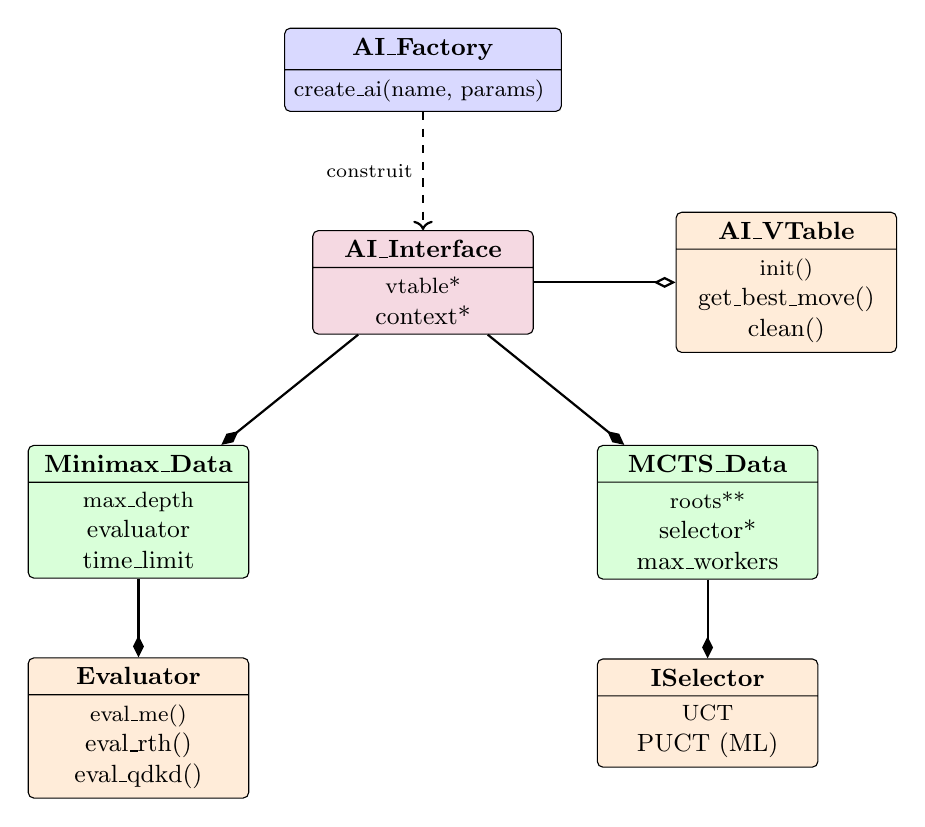
\begin{tikzpicture}[
    node distance=1.2cm and 1.8cm,
    class/.style={
        rectangle split,
        rectangle split parts=2,
        draw,
        rounded corners=2pt,
        minimum width=2.8cm,
        font=\small,
        align=center
    },
    facade/.style={class, fill=blue!15},
    context/.style={class, fill=green!15},
    data/.style={class, fill=orange!15},
    interface/.style={class, fill=purple!15},
    composition/.style={-{Diamond[fill=black]}, thick},
    aggregation/.style={-{Diamond[fill=white]}, thick},
    dependency/.style={->, dashed, thick},
]

% AI Factory (Façade centrale)
\node[facade] (factory) {
    \textbf{AI\_Factory}
    \nodepart{second}
    \footnotesize
    create\_ai(name, params)
};

% AI_Interface (Contrat public)
\node[interface, below=1.5cm of factory] (interface) {
    \textbf{AI\_Interface}
    \nodepart{second}
    \footnotesize
    vtable*\\context*
};

% VTable (Polymorphisme)
\node[data, right=1.8cm of interface] (vtable) {
    \textbf{AI\_VTable}
    \nodepart{second}
    \footnotesize
    init()\\get\_best\_move()\\clean()
};

% Implémentations concrètes
\node[context, below left=1.4cm and 0.8cm of interface] (minimax) {
    \textbf{Minimax\_Data}
    \nodepart{second}
    \footnotesize
    max\_depth\\evaluator\\time\_limit
};

\node[context, below right=1.4cm and 0.8cm of interface] (mcts) {
    \textbf{MCTS\_Data}
    \nodepart{second}
    \footnotesize
    roots**\\selector*\\max\_workers
};

% Sous-composants (Evaluators & Selectors)
\node[data, below=1cm of minimax] (eval) {
    \textbf{Evaluator}
    \nodepart{second}
    \footnotesize
    eval\_me()\\eval\_rth()\\eval\_qdkd()
};

\node[data, below=1cm of mcts] (selector) {
    \textbf{ISelector}
    \nodepart{second}
    \footnotesize
    UCT\\PUCT (ML)
};

% Relations
\draw[dependency] (factory) -- node[left, font=\scriptsize] {construit} (interface);
\draw[aggregation] (interface) -- (vtable);
\draw[composition] (interface) -- (minimax);
\draw[composition] (interface) -- (mcts);
\draw[composition] (minimax) -- (eval);
\draw[composition] (mcts) -- (selector);

% Annotations

\end{tikzpicture}
\caption{Architecture du module IA. La couche publique expose uniquement \texttt{AI\_Interface} et \texttt{AI\_Factory}. Les implémentations privées sont totalement opaques pour les appelants.}
\label{fig:ai-architecture}
\end{figure}

\subsubsection{Le patron Factory~: découplage par chaîne de caractères}

Le cœur de cette architecture repose sur le patron \textit{Factory}, qui permet de créer des instances d'IA à partir de simples chaînes de caractères. L'usine maintient un registre interne associant un nom (ex: \texttt{"mcts"}) à un constructeur. Ce mécanisme élimine tout couplage statique~:

\begin{lstlisting}[language=C, caption=Création découplée depuis l'interface publique]
// Les interfaces (CLI/GUI) ne dependent que d'une seule fonction
AI_Interface ai = create_ai("mcts", configuration_dynamique);
Move best = ai.vtable->get_best_move(&ai, game_state);
ai.vtable->clean(&ai);
\end{lstlisting}

Cette conception présente un avantage décisif lors du développement~: \textbf{un membre de l'équipe peut implémenter un nouvel algorithme sans jamais toucher au code des autres modules}. Il lui suffit de créer son fichier source, d'implémenter les fonctions de la VTable, et d'ajouter une ligne dans le registre statique de l'usine. Les interfaces supérieures continueront de l'appeler via \texttt{create\_ai} sans aucune modification.

\subsubsection{Injection de configuration par dictionnaire dynamique}

La configuration des algorithmes pose un défi architectural~: chaque IA possède des paramètres spécifiques (profondeur pour Minimax, nombre de threads pour MCTS), mais l'interface publique doit rester uniforme. 

La solution retenue est un \textbf{dictionnaire clé-valeur dynamique} (\texttt{ConfigMap}). Au lieu de passer des structures en dur, l'interface envoie un tableau de chaînes de caractères (par exemple \texttt{\{"depth", "5"\}} ou \texttt{\{"max\_workers", "8"\}}). Cette approche évite la prolifération de structures de configuration rigides et permet l'\textbf{extension sans rupture de compatibilité}. Ajouter un nouveau paramètre d'heuristique ne casse pas l'API publique~; les anciens appelants continuent de fonctionner avec les paramètres par défaut.

Pour garantir la sécurité des types à la compilation malgré l'usage de chaînes de caractères, nous utilisons le mécanisme C11 \texttt{\_Generic}. Ce dernier dispatche automatiquement le parsing vers la bonne fonction de conversion (\texttt{int}, \texttt{bool}, etc.) selon le type de la variable cible, conservant ainsi une syntaxe extrêmement propre.

\subsubsection{Récursion du patron~: Evaluators et Selectors}

Le principe de découplage par interface a été systématiquement appliqué aux \textbf{sous-composants} des algorithmes. Minimax et MCTS ne manipulent jamais directement leurs heuristiques ou stratégies de sélection.

Dans Minimax, l'évaluation du plateau est déléguée à un simple \textbf{pointeur de fonction} (\texttt{Evaluator}). Cette indirection permet de changer d'heuristique (ME, RTH, QDKD) à la volée durant les tests de performance, en modifiant uniquement la configuration d'entrée, sans toucher au code de la recherche alpha-beta.

De manière symétrique, MCTS utilise une sous-interface (\texttt{ISelector}) pour ses stratégies de sélection. Cette architecture récursive présente un avantage majeur~: \textbf{l'ajout d'une nouvelle stratégie est totalement transparent pour l'algorithme principal}. L'intégration de notre réseau de neurones (PUCT) n'a nécessité que l'implémentation de la nouvelle VTable, avec zéro modification dans le cœur du moteur MCTS.

\subsubsection{Bilan~: une architecture en poupées russes}

L'architecture finale suit un principe de \textbf{délégation en cascade}~:

\begin{center}
\texttt{CLI/GUI} $\xrightarrow{\text{crée}}$ \texttt{AI\_Factory} $\xrightarrow{\text{instancie}}$ \texttt{AI\_Interface} $\xrightarrow{\text{contient}}$ \texttt{Minimax/MCTS} $\xrightarrow{\text{utilise}}$ \texttt{Evaluator/Selector}
\end{center}

Chaque niveau ignore les détails du niveau inférieur. Cette séparation stricte a permis durant le développement~:
\begin{itemize}
    \item Le développement parallèle de Minimax et MCTS par deux membres différents de l'équipe.
    \item L'intégration tardive du machine learning (semaine 10/12) sans refonte de MCTS.
    \item Le changement d'heuristique par défaut sans modifier une seule ligne hors des fichiers dédiés.
    \item La compilation conditionnelle du support TensorFlow (\texttt{ENABLE\_ML}) sans casser les autres modules.
\end{itemize}

Cette architecture démontre qu'une conception orientée interfaces, même en C procédural, peut atteindre un niveau de modularité comparable aux langages orientés objet, tout en conservant les performances du C natif.

\subsubsection{Modélisation matricielle et source de vérité}
Afin de garantir un moteur de jeu robuste, évolutif et capable de soutenir les calculs intensifs de l'IA, l'architecture des données s'articule autour d'un modèle hybride. L'état global et officiel de la partie est encapsulé dans une structure unifiée \texttt{GameState}. La représentation structurelle de base du plateau est stockée sous forme d'un tableau dynamique à deux dimensions (matrice de type \texttt{CellContent** board}).

Cette matrice agit comme la source de vérité absolue. Chaque cellule contient une énumération définissant son état sémantique. Cette modélisation matricielle offre une lisibilité optimale pour l'interface utilisateur et permet un accès spatial direct en temps constant $\mathcal{O}(1)$. Lorsque l'IA doit évaluer l'arbre des possibles, le moteur effectue une sérialisation dynamique de cette matrice vers les structures \texttt{Bitboard}. Cette séparation des préoccupations permet de garder un code métier clair, comme l'illustre la création de l'état racine au lancement de l'algorithme~:

\begin{lstlisting}[language=C, caption=Sérialisation dynamique au lancement de la recherche]
static Move mcts_get_best_move(const AI_Interface *self, GameState state) {
    MCTS_Data *data = (MCTS_Data *)self->context;
    
    // Generation de l'etat Bitboard racine depuis la matrice UI
    BitboardState root_state = sync_from_logic(&state);
    
   
}
\end{lstlisting}

\subsubsection{Indépendance du code et encapsulation de la complexité}
Le moteur constitue le cœur logique de l'application, totalement séparé des couches d'affichage et de communication. Son code interne ne contient aucune instruction d'entrée/sortie standard (comme la lecture de fichiers) et ignore l'existence du réseau. 

Ce moteur sert de barrière stricte entre la logique mathématique du jeu et le reste du programme. La difficulté liée à la double modélisation du plateau (la matrice classique et la synchronisation des \texttt{Bitboards}) est totalement rendue invisible pour le contrôleur qui l'utilise. Il interagit avec l'extérieur exclusivement via une API minimaliste définie dans \texttt{game\_engine.h} :

\begin{lstlisting}[language=C, caption=Extrait de l'API publique du moteur masquant la complexité interne]
// Le controleur ignore l'existence des Bitboards ou de la pile Undo/Redo
bool is_move_legal(const GameState *state, Move move);
void apply_move(GameState *state, Move move);
PlayerColor get_winner(const GameState *state);
\end{lstlisting}

Lorsqu'un module (comme le CLI ou l'IA) appelle la fonction \texttt{is\_move\_legal}, le moteur s'occupe en interne de préparer les données, d'appliquer l'algorithme de lancer de rayon et de vérifier les collisions, pour finalement ne renvoyer qu'un simple booléen. 

Cette isolation forte garantit une réutilisation totale du code. Le même espace mémoire peut arbitrer une partie locale via GTK4, valider des données réseau, ou être cloné pour simuler des parties virtuelles pour l'IA, sans modification de sa structure interne.

\subsubsection{Programmation défensive et sécurité}
En tant que noyau, le moteur reçoit des appels provenant de sources variées et potentiellement imprévisibles. Chaque coordonnée envoyée est systématiquement filtrée par \texttt{is\_valid\_coord} pour empêcher les accès mémoire hors limites. Les fonctions publiques commencent par une validation des pointeurs, protégeant contre l'utilisation de données non initialisées. Cette solidité garantit que même si un autre module envoie des données corrompues, le moteur maintient son intégrité sans jamais faire planter l'application.

\subsubsection{Architecture hybride C/Python pour l'Apprentissage Automatique}

L'intégration du réseau de neurones (PUCT) repose sur une architecture hybride séparant strictement la phase d'inférence (en C) de la phase d'entraînement (en Python). Ce pont inter-langages permet d'exploiter les performances brutes du C pour la recherche arborescente, tout en bénéficiant de l'écosystème mature de Python TensorFlow/Keras pour la modélisation mathématique.

Le cycle de vie de notre modèle s'articule autour d'un pipeline de données en trois phases~:
\begin{enumerate}
    \item \textbf{Génération des données (C)~:} Le moteur C fait s'affronter des IAs (heuristique QDKD) lors de parties auto-générées (\textit{self-play}). Les états des plateaux (les tenseurs $11 \times 11 \times 4$) et les résultats finaux des parties sont sérialisés et exportés sous forme de tableaux binaires NumPy (\texttt{.npz}).
    \item \textbf{Entraînement du modèle (Python)~:} Un script ingère ces données pour entraîner le réseau de neurones. Le modèle final est exporté au format standard \textit{SavedModel}.
    \item \textbf{Inférence embarquée (C)~:} L'exécutable C charge ce modèle pré-entraîné en mémoire via l'\texttt{API C de TensorFlow}, permettant au MCTS d'interroger le réseau neuronal à la volée durant les parties.
\end{enumerate}

\paragraph{Architecture du réseau et fonction de coût.}
Contrairement à une simple régression linéaire, notre modèle est un Perceptron Multicouche (MLP). L'entrée (notre tenseur $11 \times 11 \times 4$) est d'abord aplatie (\texttt{Flatten}), puis traverse une couche cachée de 64 neurones utilisant la fonction d'activation non linéaire \texttt{ReLU}. La couche de sortie est constituée d'un neurone unique avec une activation \texttt{Sigmoïde}, contraignant la prédiction entre $0$ (défaite certaine) et $1$ (victoire certaine). 

\begin{lstlisting}[language=Python, caption=Architecture du Perceptron Multicouche (Keras)]
model = keras.Sequential([
    keras.layers.Input(shape=(11, 11, 4)),
    keras.layers.Flatten(),
    keras.layers.Dense(64, activation='relu'),   # Couche cachee
    keras.layers.Dense(1, activation='sigmoid')  # Prediction binaire
])
model.compile(optimizer='adam', loss='binary_crossentropy')
\end{lstlisting}

Le modèle est optimisé par l'algorithme \texttt{Adam}, avec pour objectif de minimiser l'erreur d'entropie croisée binaire (\texttt{Binary Cross-Entropy}), une fonction de perte parfaitement adaptée à l'évaluation de probabilités pour des problèmes de classification binaire (Gagner/Perdre).

\paragraph{Prévention du surapprentissage (\textit{Overfitting}).}
Pour garantir que l'IA développe une réelle intuition stratégique plutôt que d'apprendre bêtement les parties par cœur, nous avons implémenté une division stricte des données (80\,\% pour l'entraînement, 20\,\% pour la validation). À chaque itération (\textit{epoch}), les performances du modèle sont évaluées sur le sous-ensemble de validation qu'il n'a jamais étudié. Le suivi de ces deux courbes nous permet de trouver le point d'équilibre optimal (\textit{sweet spot}) et d'interrompre l'apprentissage avant le surapprentissage. Le script Python complet gérant ce pipeline est disponible en Annexe.

%------------------------------------------------------------------------------
% SECTION 3.4 - Architecture du module réseau
%------------------------------------------------------------------------------
 \newpage
\subsection{Architecture du module réseau}
\label{sec:network-arch}
 
L'architecture du module réseau repose sur trois piliers conceptuels~: une
façade centralisée masquant la complexité des sockets, un modèle événementiel
mono-threadé basé sur le multiplexage, et un système de rappels découplant
le cœur réseau des interfaces utilisateur. La figure~\ref{fig:network-composition}
illustre l'organisation générale de ces composants.
 
% DIAGRAMME 1 : Composition du NetworkManager
\begin{figure}[H]
\centering
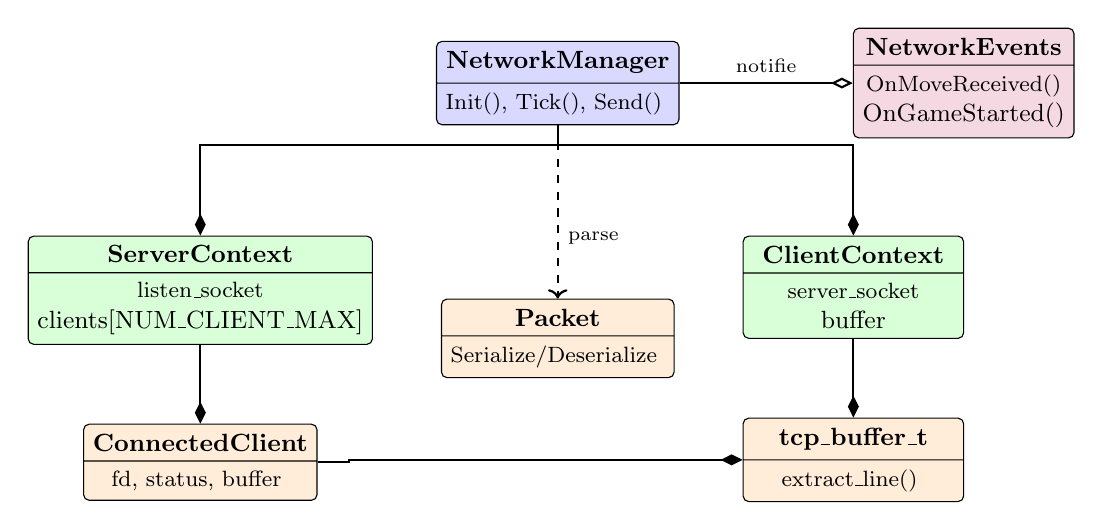
\begin{tikzpicture}[
    node distance=1.2cm and 1.8cm,
    class/.style={
        rectangle split,
        rectangle split parts=2,
        draw,
        rounded corners=2pt,
        minimum width=2.8cm,
        font=\small,
        align=center
    },
    facade/.style={class, fill=blue!15},
    context/.style={class, fill=green!15},
    data/.style={class, fill=orange!15},
    interface/.style={class, fill=purple!15},
    composition/.style={-{Diamond[fill=black]}, thick},
    aggregation/.style={-{Diamond[fill=white]}, thick},
    dependency/.style={->, dashed, thick},
]
 
% NetworkManager (Façade)
\node[facade] (nm) {
    \textbf{NetworkManager}
    \nodepart{second}
    \footnotesize
    Init(), Tick(), Send()
};
 
% Contextes
\node[context, below left=1.4cm and 0.8cm of nm] (server) {
    \textbf{ServerContext}
    \nodepart{second}
    \footnotesize
   listen\_socket\\clients[NUM\_CLIENT\_MAX]
};
 
\node[context, below right=1.4cm and 0.8cm of nm] (client) {
    \textbf{ClientContext}
    \nodepart{second}
    \footnotesize
    server\_socket\\buffer
};
 
% ConnectedClient
\node[data, below=1cm of server] (cc) {
    \textbf{ConnectedClient}
    \nodepart{second}
    \footnotesize
    fd, status, buffer
};
 
% tcp_buffer_t
\node[data, below=1cm of client] (buffer) {
    \textbf{tcp\_buffer\_t}
    \nodepart{second}
    \footnotesize
    extract\_line()
};
 
% NetworkEvents (Observateur)
\node[interface, right=2.2cm of nm] (events) {
    \textbf{NetworkEvents}
    \nodepart{second}
    \footnotesize
    OnMoveReceived()\\OnGameStarted()
};
 
% Packet
\node[data, below=2.2cm of nm] (packet) {
    \textbf{Packet}
    \nodepart{second}
    \footnotesize
    Serialize/Deserialize
};
 
% Relations
\draw[composition] (nm.south) -- ++(0,-0.25) -| (server.north);
\draw[composition] (nm.south) -- ++(0,-0.25) -| (client.north);
\draw[composition] (server.south) -- (cc.north);
\draw[composition] (client.south) -- (buffer.north);
\draw[composition] (cc.east) -- ++(0.4,0) |- (buffer.west);
\draw[aggregation] (nm.east) -- node[above, font=\scriptsize] {notifie} (events.west);
\draw[dependency] (nm.south) -- node[right, font=\scriptsize, pos=0.65] {parse} (packet.north);
 
\end{tikzpicture}
\caption{Diagramme de composition du \texttt{NetworkManager}. La façade possède
au plus un contexte serveur \textbf{ou} client (exclusion mutuelle). Chaque
client embarque son propre tampon TCP. Légende~: $\blacklozenge$ composition,
$\lozenge$ agrégation, trait pointillé = dépendance.}
\label{fig:network-composition}
\end{figure}
 
\subsubsection{La façade \texttt{NetworkManager}}
\label{subsec:facade}
 
\paragraph{}
Le module réseau expose une unique structure publique --- \texttt{NetworkManager}
--- qui encapsule l'intégralité de la logique de communication. Les couches
supérieures (CLI, GUI) n'ont jamais besoin de manipuler directement les
descripteurs de fichiers, les structures d'adresses réseau, ni les tampons
de framing. Ce masquage strict de l'information garantit que toute évolution
interne (passage à TLS, changement de protocole) n'impacte pas le code client.

L'initialisation de la façade illustre cette encapsulation~:

\begin{lstlisting}[language=C, caption=Initialisation du NetworkManager]
void NetworkManager_Init(NetworkManager *manager, NetworkEvents callbacks) {
  manager->current_mode = NET_MODE_NONE;
  manager->server_ctx = NULL;
  manager->client_ctx = NULL;
  manager->callbacks = callbacks;  // Injection des rappels
}
\end{lstlisting}
 
\paragraph{}
Le \texttt{NetworkManager} peut fonctionner en trois modes mutuellement
exclusifs~: inactif, serveur ou client. En mode serveur, il alloue un
\texttt{ServerContext} contenant la socket d'écoute, le tableau des 64 slots
clients avec leurs tampons TCP respectifs, le tableau des 32 parties actives,
et le contexte de découverte UDP. En mode client, il alloue un
\texttt{ClientContext} minimaliste contenant uniquement la socket de connexion
au serveur et son tampon de réception. Cette ségrégation mémoire évite toute
confusion entre les rôles et permet une libération ciblée des ressources.
 
\subsubsection{Le multiplexage asynchrone avec \texttt{poll()}}
\label{subsec:multiplexing}
 
\paragraph{}
Pour gérer simultanément jusqu'à 64 connexions sans threads, nous avons opté
pour le multiplexage d'entrées/sorties via l'appel système \texttt{poll()}.
Trois alternatives existaient~: \texttt{select()}, limité à 1\,024 descripteurs
et utilisant des masques de bits peu pratiques~; \texttt{epoll()}, plus
performant mais spécifique à Linux~; et \texttt{poll()}, offrant une interface
portable POSIX avec des performances adaptées à notre charge. Le modèle
mono-threadé élimine par construction les conditions de course et la nécessité
de verrous, simplifiant considérablement le raisonnement sur la correction
du code.
 
\paragraph{}
La fonction \texttt{NetworkManager\_Tick()}, appelée à chaque itération de la
boucle principale, invoque \texttt{poll()} avec un timeout nul. Ce paramétrage
rend l'appel instantanément retourné~: si des données sont disponibles, elles
sont traitées~; sinon, le contrôle revient immédiatement à l'appelant. Cette
conception permet à l'interface de continuer à traiter d'autres événements
(saisie clavier, rafraîchissement graphique) entre deux cycles réseau.

\begin{lstlisting}[language=C, caption=Tick serveur avec poll() non bloquant]
static void handle_server_tick(NetworkManager *manager, ServerContext *ctx) {
  int poll_count = poll(ctx->fds, MAX_CLIENTS + 1, POLL_TIMEOUT_IMMEDIATE);
  
  if (poll_count > 0) {
    if (ctx->fds[LISTEN_SOCKET_INDEX].revents & POLLIN)
      handle_server_new_connection(ctx);
    
    for (int i = FIRST_CLIENT_INDEX; i <= MAX_CLIENTS; i++) {
      if (ctx->fds[i].fd != INVALID_SOCKET &&
          (ctx->fds[i].revents & (POLLIN | POLLHUP | POLLERR)))
        handle_server_client_data(manager, ctx, i);
    }
  }
}
\end{lstlisting}
 
\paragraph{}
La boucle principale du CLI illustre une application avancée de ce modèle~:
elle doit surveiller simultanément deux sources d'événements indépendantes
--- le réseau et le clavier. Plutôt que de créer deux threads ou de bloquer
sur l'une des sources, nous utilisons deux appels \texttt{poll()} distincts
à chaque itération~: le premier interroge les sockets réseau avec un timeout
nul (traitement immédiat des paquets entrants), le second interroge
\texttt{stdin} avec un court timeout permettant la saisie de commandes. Cette
architecture permet au joueur de taper des commandes tout en recevant
instantanément les coups de l'adversaire, simulant un parallélisme sans les
risques inhérents à la programmation concurrente.
 
\subsubsection{Le patron Observateur pour le découplage}
\label{subsec:observer}
 
\paragraph{}
La communication entre le module réseau et les couches supérieures est régie
par le patron \textit{Observer}. À l'initialisation, le \texttt{NetworkManager}
reçoit une structure \texttt{NetworkEvents} contenant neuf pointeurs de
fonctions couvrant tous les événements significatifs~: réception d'un coup,
connexion ou déconnexion d'un joueur, réception d'une invitation, démarrage
d'une partie, erreur protocolaire, expiration du temps de réflexion, et
réception d'une liste de joueurs.
 
\paragraph{}
Lorsque le réseau reçoit un coup valide, il se contente d'invoquer le rappel
\texttt{OnMoveReceived(move)} sans connaître l'identité de l'appelant. C'est
la couche d'interface qui décide de la réaction appropriée~: le CLI met à jour
l'affichage textuel du plateau et réaffiche le prompt, tandis que la GUI
redessine les cases concernées via les primitives GTK. Cette inversion de
contrôle garantit que le module réseau reste totalement indépendant des
interfaces utilisateur~: les fichiers d'implémentation CLI et GUI fournissent
chacun leur propre jeu de rappels sans qu'une seule ligne du cœur réseau
n'ait été modifiée.
 
\subsubsection{Routage des paquets et arbitrage serveur}
\label{subsec:routing}
 
\paragraph{}
Une fois un paquet désérialisé, il est acheminé vers un gestionnaire dédié
via une structure de sélection indexée par le type de paquet. Cette conception
respecte le principe ouvert/fermé~: ajouter un nouveau type de message
nécessite uniquement l'ajout d'un cas dans le gestionnaire, sans modifier
la logique de routage existante.

\begin{lstlisting}[language=C, caption=Routage des paquets par type]
void handle_server_packet(NetworkManager *manager, ServerContext *ctx,
                          int client_index, Packet *pkt) {
  switch (pkt->type) {
    case C2S_JOIN:   process_join_packet(manager, ctx, client_index, pkt->payload); break;
    case C2S_INVITE: process_invite_packet(manager, ctx, client_index, pkt->payload); break;
    case C2S_MOVE:   process_move_packet(manager, ctx, client_index, pkt->payload); break;
    case C2S_HEARTBEAT: break;  // Mise a jour silencieuse du timestamp
    // ... autres cas
    default: printf("[SERVER] Unmanaged packet (Type: %d)\n", pkt->type);
  }
}
\end{lstlisting}
 
\paragraph{}
Le serveur ne se contente pas de relayer aveuglément les coups entre joueurs.
Avant tout transfert, il maintient une copie locale du plateau pour chaque
partie active et valide la légalité de chaque coup reçu. Si un coup est
déterminé illégal par le moteur de jeu, il est rejeté avec un message d'erreur
explicite envoyé au client fautif, et l'adversaire n'est jamais notifié de
cette tentative. Ce mécanisme garantit qu'un client malveillant ou bogué ne
peut pas corrompre l'état de jeu de son adversaire ni obtenir un avantage
indu.

\begin{lstlisting}[language=C, caption=Validation anti-triche des coups]
// Extrait de process_move_packet()
GameState *server_board = &ctx->active_games[game_idx];

if (is_move_legal(server_board, parsed_move)) {
  apply_move(server_board, parsed_move);  // MAJ plateau arbitre
  // Relais vers l'adversaire...
} else {
  printf("[ANTI-CHEAT] Client %d tried illegal move\n", client_index);
  send_error(manager, client_index, "Illegal move detected!");
}
\end{lstlisting}

 
\paragraph{}
Chaque partie active possède un identifiant unique attribué séquentiellement
par le serveur. Lorsqu'un client envoie un coup, le serveur consulte son
champ \texttt{game\_id} pour identifier la partie concernée, puis parcourt
les clients connectés pour trouver celui partageant le même identifiant avec
un statut «~en jeu~». Cette recherche, bien que linéaire dans le pire cas
($\mathcal{O}(n)$ où $n$ est le nombre de clients), reste négligeable en
pratique car le nombre de clients actifs est borné.


\subsubsection{Structures de contexte et gestion des connexions}
\label{subsec:context-structures}
 
\paragraph{}
Chaque client est représenté par une structure à taille fixe regroupant
l'ensemble des informations nécessaires à sa gestion~: le descripteur de
socket, son tampon TCP dédié, son pseudo, son statut courant dans la machine
à états, l'identifiant de sa
partie en cours, l'horodatage de sa dernière activité, et les métadonnées
d'invitation pendante. Cette encapsulation permet de traiter chaque client
comme une entité autonome sans variables globales partagées.
 
\paragraph{}
Une décision architecturale majeure concerne l'allocation mémoire~: les 64
slots clients et les 32 slots de parties sont alloués \textbf{une seule fois}
au démarrage du serveur. Aucune allocation dynamique n'intervient lors des
connexions ou déconnexions~: un client qui se connecte occupe un slot
précédemment marqué invalide, et sa déconnexion remet simplement ce marqueur.
Ce patron de \textit{pool d'objets} présente trois avantages~: il élimine
la fragmentation mémoire sur les serveurs à longue durée de vie, il garantit
un temps de traitement constant par connexion ($\mathcal{O}(1)$ pour trouver
un slot libre dans le pire cas via parcours linéaire borné), et il rend
l'empreinte mémoire totale déterministe et prévisible dès le démarrage.
 
\paragraph{}
Une optimisation critique réside dans l'alignement des tableaux de surveillance
et de métadonnées~: l'index $i$ dans le tableau \texttt{fds[]} utilisé par
\texttt{poll()} correspond \textbf{exactement} à l'index $i$ dans le tableau
\texttt{clients[]}. Cette correspondance bijective permet de passer en
$\mathcal{O}(1)$ du descripteur de fichier signalé par le système d'exploitation
aux informations complètes du joueur (pseudo, statut, partie en cours), sans
recourir à une recherche linéaire ou à une table de hachage. L'index 0 est
réservé à la socket d'écoute du serveur, les index 1 à 64 correspondent aux
clients connectés.

\subsubsection{Sérialisation et framing TCP}
\label{subsec:serialization}

\paragraph{}
Chaque paquet suit le format textuel \texttt{"TYPE|PAYLOAD\textbackslash{}n"}. La sérialisation et désérialisation s'effectuent en temps linéaire par rapport à la taille du message~:

\begin{lstlisting}[language=C, caption=Sérialisation des paquets]
int SerializePacket(const Packet *pkt, char *buffer_out, size_t max_len) {
  return snprintf(buffer_out, max_len, "%d|%s\n", pkt->type, pkt->payload);
}
\end{lstlisting}

\paragraph{}
Le tampon TCP accumule les fragments jusqu'à réception d'un délimiteur \texttt{'\textbackslash{}n'}. L'extraction utilise \texttt{memchr()} pour la recherche et \texttt{memmove()} pour la compaction~:

\begin{lstlisting}[language=C, caption=Extraction d'une ligne du tampon TCP]
int tcp_buffer_extract_line(tcp_buffer_t *buf, char *out_msg, size_t max_len) {
  char *newline = memchr(buf->data, '\n', buf->length);
  if (newline == NULL) return EXTRACT_NO_MSG;
  
  size_t msg_len = newline - buf->data;
  memcpy(out_msg, buf->data, msg_len);
  out_msg[msg_len] = '\0';
  
  size_t remaining = buf->length - msg_len - 1;
  memmove(buf->data, newline + 1, remaining);  // Compaction
  buf->length = remaining;
  return EXTRACT_SUCCESS;
}
\end{lstlisting}
\newpage
\subsection{Le module d'interface graphique (GUI)}
\label{sec:gui-arch}

L'architecture du module graphique, mise en place avec la bibliothèque GTK4~\cite{gtk4doc}, a été conçue selon le pattern \textbf{Modèle-Vue-Contrôleur (MVC)}. L'enjeu principal de ce module consistait à interfacer une boucle d'événements purement asynchrone avec un moteur de jeu déterministe et des services potentiellement bloquants (Réseau, Intelligence Artificielle). La figure~\ref{fig:gui_architecture} présente l'architecture autour de la GUI.

% DIAGRAMME ARCHITECTURE GUI
\begin{figure}[H]
\centering
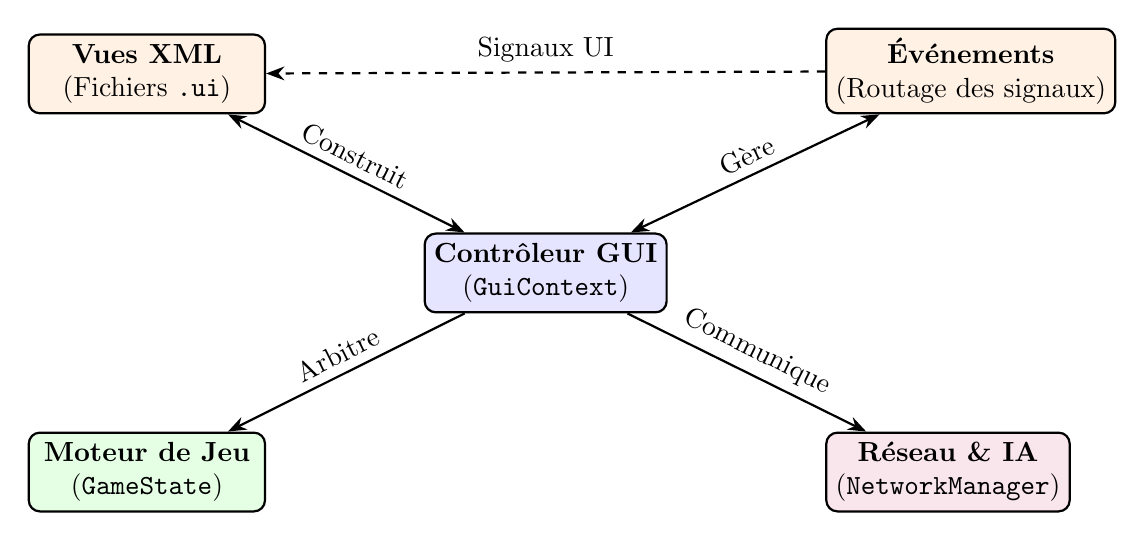
\begin{tikzpicture}[
    node distance=1.5cm and 2cm,
    module/.style={rectangle, draw, rounded corners, fill=blue!10, thick, minimum width=3cm, minimum height=1cm, align=center},
    view/.style={rectangle, draw, rounded corners, fill=orange!10, thick, minimum width=3cm, minimum height=1cm, align=center},
    arrow/.style={->, thick, >=Stealth}
]

% Nodes
\node[module] (controller) {\textbf{Contrôleur GUI}\\(\texttt{GuiContext})};
\node[view, above left=of controller] (pages) {\textbf{Vues XML}\\(Fichiers \texttt{.ui})};
\node[view, above right=of controller] (callbacks) {\textbf{Événements}\\(Routage des signaux)};
\node[module, fill=green!10, below left=of controller] (engine) {\textbf{Moteur de Jeu}\\(\texttt{GameState})};
\node[module, fill=purple!10, below right=of controller] (network) {\textbf{Réseau \& IA}\\(\texttt{NetworkManager})};

% Arrows
\draw[arrow, <->] (controller) -- node[above, sloped] {Construit} (pages);
\draw[arrow, <->] (controller) -- node[above, sloped] {Gère} (callbacks);
\draw[arrow, dashed] (callbacks) -- node[above] {Signaux UI} (pages);
\draw[arrow] (controller) -- node[above, sloped] {Arbitre} (engine);
\draw[arrow] (controller) -- node[above, sloped] {Communique} (network);

\end{tikzpicture}
\caption{Architecture du module graphique~: le contrôleur orchestre les vues asynchrones, le réseau et le modèle de jeu.}
\label{fig:gui_architecture}
\end{figure}

\subsubsection{Séparation déclarative et encapsulation des ressources}

L'interface visuelle est dissociée du code C via des fichiers de description déclarative au format XML (fichiers \texttt{.ui}). Cette séparation présente un double avantage~: elle permet la modification de la topologie de l'interface sans recompilation de la logique applicative, et elle concentre l'initialisation du code sur l'injection de dépendances (\textit{event binding}) via \texttt{GtkBuilder}. 

Pour garantir la portabilité de l'exécutable, ces ressources XML (ainsi que les feuilles de style CSS) sont compilées nativement dans le binaire final via le système \texttt{GResource}. L'application est ainsi livrée sous forme d'un exécutable autonome ( \textit{standalone}), éliminant les risques liés aux chemins de fichiers relatifs manquants sur la machine cible.

\subsubsection{L'orchestrateur asynchrone et la Main Loop}

Le défi majeur d'une interface graphique développée en C est le syndrome de l'interface figée (\textit{UI freeze}). Le système de fenêtrage repose sur une boucle principale (\textit{Main Loop}) qui ne doit jamais être bloquée.

Pour y parvenir, le contrôleur \texttt{GuiContext} agit comme un \textbf{orchestrateur asynchrone}. Les opérations légères mais récurrentes (comme le \texttt{Tick()} du gestionnaire réseau) sont greffées sur la boucle GTK via des \textit{timeouts} (\texttt{g\_timeout\_add}). À l'inverse, les calculs lourds d'IAs sont instanciés dans des \textit{threads} POSIX parallèles (\texttt{g\_thread\_new}). Pour garantir la \textit{thread-safety} absolue lors du rafraîchissement visuel, le thread d'IA utilise la primitive \texttt{g\_idle\_add} pour réinjecter de manière sécurisée son résultat (le meilleur coup calculé) dans le thread principal de GTK. De plus, des conditions bloquent totalement certaines actions qui pourraient corrompre la partie en cours si le thread de l'IA est actuellement actif. L'interface reste ainsi fluide et réactive en toutes circonstances.

\subsubsection{Automate fini interactif et approche transactionnelle}

Contrairement aux échecs, un tour aux Amazones est une transaction en deux temps (déplacement, puis tir). Pour empêcher toute corruption de l'état du jeu par des clics erratiques, les interactions avec le plateau (clics et \textit{Drag \& Drop} natif via \texttt{GtkDragSource} / \texttt{GtkDropTarget}) sont régies par une \textbf{machine à états finis (FSM)} stricte.

Le système oscille entre \texttt{PHASE\_MOVE\_QUEEN} et \texttt{PHASE\_SHOOT\_ARROW}. Lors du déplacement de la reine, l'interface adopte une approche \textbf{transactionnelle retardée}~: le déplacement n'est opéré qu'en mémoire graphique locale pour fournir un retour visuel immédiat à l'utilisateur. La méthode de mutation officielle de l'état du noyau (\texttt{apply\_move}) n'est invoquée qu'à l'issue complète de la transaction (validation du tir de la flèche). Ainsi, le moteur central et sa pile d'historique (Undo/Redo) ne reçoivent jamais d'états partiels ou corrompus. En cas d'annulation par clic droit durant la phase de tir, la transaction graphique est simplement avortée (\textit{rollback} visuel).

\subsubsection{Navigation lâche et stylisation dynamique}

La gestion de la navigation entre les différents écrans (Menu, Jeu, Lobby, Configuration) s'articule autour d'un conteneur \texttt{GtkStack}. Le contrôleur utilise un couplage lâche~: plutôt que de coder en dur les transitions, les boutons de l'interface intègrent l'identifiant de leur page cible directement dans leurs balises XML personnalisées. Le contrôleur se contente de router génériquement ces requêtes.

Enfin, la clarté visuelle du plateau de jeu est assurée par un \texttt{GtkCssProvider}. Au lieu de manipuler pixel par pixel la couleur des cases, le contrôleur applique et retire dynamiquement des classes CSS sémantiques (\texttt{.piece-white}, \texttt{.highlight-valid}, \texttt{.hint-arrow}). Cette approche permet non seulement de thématiser l'application en un instant, mais délègue surtout le moteur de rendu au processeur graphique (GPU) interne de GTK4, assurant des animations et des mises en surbrillance d'une grande fluidité.




\subsection{Architecture du module CLI}
\label{sec:cli-arch}

Le module CLI a été conçu selon des principes stricts de séparation des préoccupations, garantissant que la logique d'interface n'interfère jamais avec les règles du moteur de jeu. 

\begin{figure}[H]
\centering
\resizebox{\textwidth}{!}{%
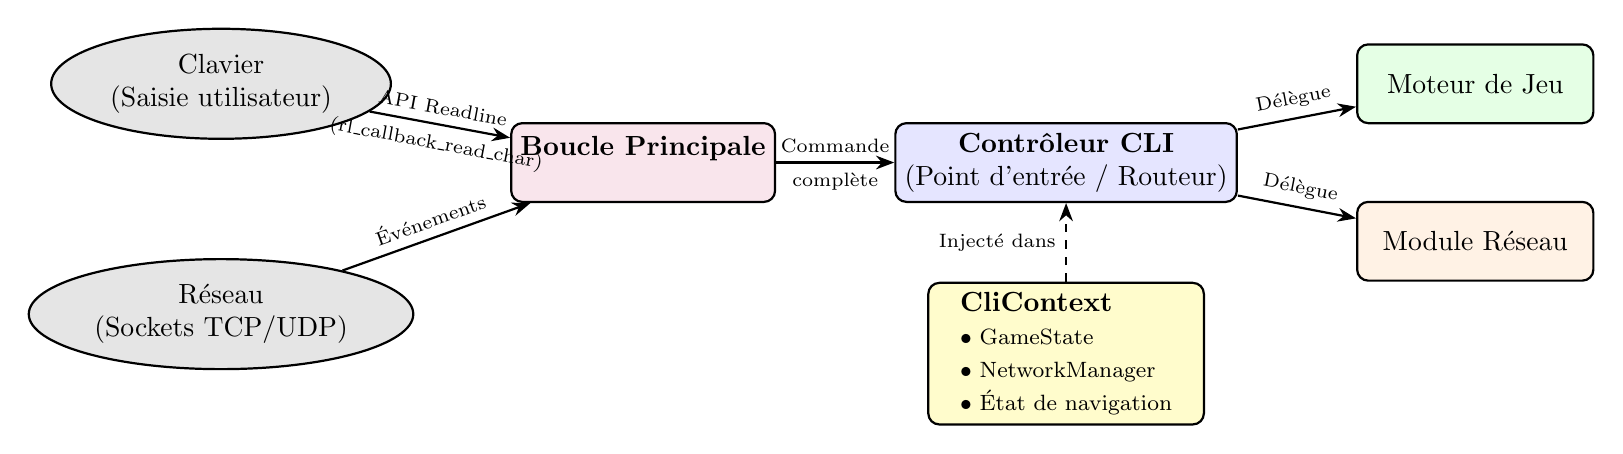
\begin{tikzpicture}[
    node distance=1.5cm and 1.5cm,
    module/.style={rectangle, draw, rounded corners, thick, minimum width=3cm, minimum height=1cm, align=center, fill=blue!10},
    context/.style={rectangle, draw, rounded corners, thick, minimum width=3.5cm, minimum height=1.5cm, align=left, fill=yellow!20},
    input/.style={ellipse, draw, thick, align=center, fill=gray!20, minimum width=2.5cm},
    arrow/.style={->, thick, >=Stealth}
]

\node[input] (keyboard) {Clavier\\(Saisie utilisateur)};
\node[input, below=1.5cm of keyboard] (network_in) {Réseau\\(Sockets TCP/UDP)};

% Boucle Principale (espacement réduit à 1.5cm)
\node[module, fill=purple!10, right=1.5cm of keyboard, yshift=-1cm] (mainloop) {\textbf{Boucle Principale}\\};

% Contrôleur (Routeur)
\node[module, right=1.5cm of mainloop] (router) {\textbf{Contrôleur CLI}\\(Point d'entrée / Routeur)};

% Contexte (Encapsulation)
\node[context, below=1cm of router] (clicontext) {\textbf{CliContext}\\ \footnotesize $\bullet$ GameState \\ \footnotesize $\bullet$ NetworkManager \\ \footnotesize $\bullet$ État de navigation};

% Sous-modules (Délégation)
\node[module, fill=green!10, right=1.5cm of router, yshift=1cm] (engine) {Moteur de Jeu};
\node[module, fill=orange!10, right=1.5cm of router, yshift=-1cm] (network_out) {Module Réseau};

% Flèches et relations
\draw[arrow] (keyboard) -- node[above, sloped, font=\scriptsize] {API Readline} node[below, sloped, font=\scriptsize] {(rl\_callback\_read\_char)} (mainloop);
\draw[arrow] (network_in) -- node[above, sloped, font=\scriptsize] {Événements} (mainloop);

\draw[arrow] (mainloop) -- node[above, font=\scriptsize] {Commande} node[below, font=\scriptsize] {complète} (router);

\draw[arrow, dashed] (clicontext) -- node[left, font=\scriptsize] {Injecté dans} (router);

\draw[arrow] (router) -- node[above, sloped, font=\scriptsize] {Délègue} (engine);
\draw[arrow] (router) -- node[above, sloped, font=\scriptsize] {Délègue} (network_out);

\end{tikzpicture}%
}
\caption{Architecture du module CLI : intégration asynchrone des entrées, routage centralisé et encapsulation de l'état d'exécution.}
\label{fig:cli_architecture}
\end{figure}

\subsubsection{Le contexte CLI (\texttt{CliContext}) et le routage centralisé}
Pour éviter les variables globales, l'ensemble de l'état de la session est centralisé dans une structure \texttt{CliContext} transmise à chaque fonction. Cette structure agit comme un patron de conception \textit{State} : elle regroupe le pointeur vers la partie en cours, l'état de navigation (menu, lobby réseau, en jeu), les instances d'IA et le gestionnaire réseau.

L'analyse des commandes fonctionne sur le principe d'un routeur centralisé. L'algorithme isole le premier mot saisi et le compare à un dictionnaire de commandes via des constantes symboliques. L'exécution finale dépend de la validation de l'état présent dans le \texttt{CliContext}. Le contrôleur peut ainsi bloquer des commandes illogiques (ex: empêcher \texttt{undo} en partie multijoueur) sans jamais solliciter le moteur de jeu.

\subsubsection{Boucle événementielle hybride et multiplexage}
Le contrôleur CLI implémente une boucle principale non bloquante devant surveiller simultanément le clavier et le réseau. Plutôt que de recourir au multi-threading complexe, nous utilisons un double multiplexage avec \texttt{poll()}. 

À chaque itération, un premier \texttt{poll()} réseau avec un timeout nul traite instantanément les paquets entrants. Ensuite, la logique de jeu (fin de partie, tour IA, timeout) est évaluée. Enfin, un second \texttt{poll()} interroge l'entrée standard (\texttt{stdin}) avec un timeout court. Cette architecture permet au joueur de saisir des commandes tout en recevant les coups de l'adversaire en temps réel, simulant un parallélisme robuste.

\subsubsection{Sérialisation et robustesse du parsing}
La persistance des données (sauvegarde/chargement) repose sur une analyse syntaxique séquentielle en temps linéaire $\mathcal{O}(N)$. Avant l'analyse, chaque ligne subit un pré-traitement strict filtrant les commentaires (\texttt{\{} ou \texttt{\#}) et les espaces redondants, protégeant l'application contre les fichiers au formatage capricieux.

L'analyseur maintient une variable d'état pour s'orienter entre les sections (paramètres, plateau, historique). Cette conception impose une sécurité d'ordre logique : la dimension du plateau doit impérativement être validée dans les paramètres avant d'allouer la matrice ou de reconstruire l'historique, empêchant toute corruption mémoire.

\subsubsection{Validation mathématique et sécurité des entrées}
La conversion de la notation algébrique standard (ex: \texttt{d4}) en coordonnées cartésiennes $(x, y)$ constitue une ultime barrière de sécurité. Pour un plateau $D \times D$, la conversion s'effectue par des soustractions sur l'ordre alphabétique :
$$x = \text{lettre} - \text{'a'} \qquad y = \text{chiffre} - 1$$

Une validation stricte des bornes $(0 \le x < D) \land (0 \le y < D)$ est appliquée immédiatement. Cette vérification mathématique empêche les dépassements de capacité inhérents aux variables non signées en cas de résultat négatif. Le moteur de jeu ne reçoit ainsi que des instructions préalablement assainies.


%==============================================================================
\section{Explication approfondie}
\label{sec:deep}
%==============================================================================

 
%------------------------------------------------------------------------------
% SECTION 4.1 - Cycle de vie des connexions
%------------------------------------------------------------------------------
 
%------------------------------------------------------------------------------
% SECTION 4.1 - REMPLACE l'ancienne section "Cycle de vie des connexions"
%------------------------------------------------------------------------------
 
\subsection{Fonctionnalité réseau~: Système d'invitations et machine à états (F40)}
\label{subsec:network-invitations}
 
\subsubsection{Prérequis et problème}
 
Le cahier des charges (F40) impose un système complet d'invitations permettant aux joueurs de se défier dans le lobby. Ce système doit gérer plusieurs cas complexes~: un joueur peut être indisponible (\texttt{AWAY}), déjà en partie (\texttt{INGAME}), ou en attente de réponse (\texttt{WAITGAME}). Les invitations doivent expirer automatiquement après 5 minutes, et toute transition d'état invalide doit être rejetée avec un message explicite.
 
\subsubsection{Solution implémentée~: machine à états finis}
 
Nous avons modélisé le cycle de vie d'un client par un automate fini à cinq états. Chaque transition est gardée par des vérifications explicites~:
 
\begin{lstlisting}[language=C, caption=Énumération des statuts clients]
typedef enum {
  CLIENT_STATUS_CONNECTED,  // TCP etabli, attente JOIN
  CLIENT_STATUS_IDLE,       // Dans le lobby, disponible
  CLIENT_STATUS_AWAY,       // Indisponible temporairement
  CLIENT_STATUS_WAITGAME,   // Invitation en attente
  CLIENT_STATUS_INGAME      // Partie en cours
} ClientStatus;
\end{lstlisting}
 
\paragraph{Traitement d'une invitation.}
Lorsqu'un joueur envoie une invitation, le serveur vérifie l'éligibilité via des gardes d'état~:
 
\begin{lstlisting}[language=C, caption=Gardes de transition pour les invitations]
// Extrait de process_invite_packet()
if (ctx->clients[sender_index].status != CLIENT_STATUS_IDLE) {
  send_error(manager, sender_index, "You must be IDLE to invite.");
  return;
}
if (ctx->clients[target_id].status == CLIENT_STATUS_AWAY) {
  send_error(manager, sender_index, "Player is currently AWAY.");
  return;
}
// Transitions d'etat apres validation
ctx->clients[sender_index].status = CLIENT_STATUS_WAITGAME;
ctx->clients[target_id].pending_invite_from = sender_index;
\end{lstlisting}
 
\paragraph{Expiration automatique.}
À chaque tick serveur, les invitations pendantes sont vérifiées. Une invitation non répondue après 300 secondes déclenche le retour au statut \texttt{IDLE} pour les deux joueurs avec notification explicite.
 
\subsubsection{Garanties de cohérence}
 
Cette implémentation garantit trois propriétés~: \textbf{déterminisme} (chaque paquet produit exactement une transition ou un rejet), \textbf{isolation} (un joueur en partie ne peut recevoir d'invitations), et \textbf{récupération automatique} (les timeouts libèrent les ressources bloquées).
 
\newpage
\subsection{Fonctionnalité 2~: Approfondissement itératif avec contrainte de temps}
\label{subsec:iterative-deepening}

\subsubsection{Prérequis et problème}

L'algorithme Minimax classique explore l'arbre de jeu jusqu'à une profondeur fixe $d$, puis retourne le meilleur coup trouvé. Cette approche présente un défaut majeur~: si $d$ est trop grand, le calcul peut dépasser le temps imparti, ne retournant aucun coup valide. Si $d$ est trop petit, l'IA joue de manière myope. Le cahier des charges (F34) impose donc un mécanisme garantissant le retour du \textbf{meilleur coup trouvé à la profondeur maximale complétée} avant l'expiration du délai.

\subsubsection{Solution implémentée~: Iterative Deepening}

L'approfondissement itératif consiste à explorer l'arbre en profondeur croissante ($d = 1, 2, 3, \ldots$) jusqu'à épuisement du temps. À chaque itération complète, le meilleur coup est mis à jour. Si le temps expire en milieu d'exploration, le coup de l'itération précédente est retourné.

\paragraph{Implémentation.}
La fonction \texttt{minimax\_get\_best\_move} contient une boucle principale~:

\begin{lstlisting}[language=C, caption=Boucle d'approfondissement itératif]
Move best_move_overall = available_moves[0];

for (int d = 1; d <= data->max_depth; d++) {
    if (get_time_ms() - start_time >= data->time_limit)
        break;
    
    // Tri des coups pour placer le meilleur de l'iteration
    // precedente en tete (ameliore le pruning)
    if (d > 1)
        sort_moves(count, best_move_overall, available_moves);
    
    Move move_at_depth = run_root_search(data, &root_state, d, 
                                         start_time, available_moves, count);
    
    // Sauvegarde uniquement si l'iteration s'est terminee
    if (get_time_ms() - start_time < data->time_limit) {
        best_move_overall = move_at_depth;
    }
}

return best_move_overall;
\end{lstlisting}

\paragraph{Optimisation par réordonnancement des coups.}
Avant chaque nouvelle profondeur, la fonction \texttt{sort\_moves} place le meilleur coup de l'itération précédente en tête du tableau. Cette heuristique exploite le fait que le coup optimal à profondeur $d-1$ est souvent proche de celui à profondeur $d$, ce qui améliore significativement l'efficacité de l'élagage alpha-beta en explorant d'abord les branches prometteuses.

\paragraph{Garanties temporelles.}
La vérification \texttt{get\_time\_ms() - start\_time < data->time\_limit} est effectuée~:
\begin{itemize}
    \item Avant chaque nouvelle itération de profondeur
    \item À l'intérieur de \texttt{alpha\_beta\_forward} avant chaque expansion de nœud
    \item Avant la sauvegarde du meilleur coup
\end{itemize}

Cette triple vérification garantit que l'algorithme ne dépasse jamais le temps alloué de plus de quelques millisecondes (le temps d'une seule expansion de nœud).

\subsubsection{Intégration avec Forward Pruning (F33)}

Lorsque le forward pruning est activé, chaque itération de profondeur bénéficie d'un faisceau de recherche adaptatif. La largeur du faisceau croît avec la profondeur restante~:

\begin{lstlisting}[language=C]
int get_beam_width(int maximizing, int current_depth, int max_depth) {
    int base = maximizing ? NB_BEST_MOVES_PLAYER : NB_BEST_MOVES_OPPONENT;
    int depth_bonus = (max_depth - current_depth) * 3;
    return base + depth_bonus;
}
\end{lstlisting}

Ainsi, à profondeur 1, seuls 10 coups sont explorés (joueur maximisant), mais à profondeur 5 avec $d_{\max} = 5$, le faisceau s'élargit à $10 + (5-1) \times 3 = 22$ coups. Cette approche équilibre vitesse (petits faisceaux en profondeur) et précision (faisceaux larges près de la racine).


%==============================================================================
\section{Stratégie de test et assurance qualité}
\label{sec:tests}
%==============================================================================
 
La fiabilité d'un projet de cette envergure ne peut reposer uniquement sur
des vérifications manuelles. Nous avons mis en place une chaîne complète
d'assurance qualité intégrant tests unitaires, couverture de code, analyse
statique, vérification de style et documentation embarquée. Cette section
détaille chacun de ces piliers.
 
\subsection{Framework de test~: GoogleTest}
 
L'ensemble des tests repose sur le framework \textbf{GoogleTest}
(v1.15.2), téléchargé et compilé automatiquement par CMake
via \texttt{FetchContent}. Bien que notre code source soit intégralement écrit
en C, GoogleTest est un framework C++~: chaque fichier de test inclut donc
les en-têtes C au sein de blocs \texttt{extern "C" \{\}} pour assurer une
interopérabilité transparente entre les deux langages. Ce choix nous offre
l'expressivité des macros \texttt{TEST}, \texttt{TEST\_F},
\texttt{EXPECT\_EQ}, \texttt{EXPECT\_TRUE}, etc., tout en testant du code C
pur sans modification.
 
Au total, le projet comporte \textbf{plus de 600 cas de test} répartis dans
\textbf{25 fichiers}, couvrant l'ensemble des modules de l'application.
 
 
\subsection{Infrastructure de test~: fixtures et mocks}
 
Pour les modules dont l'initialisation requiert un état complexe, nous avons
développé des \textbf{fixtures de test} (classes héritant de
\texttt{::testing::Test}) qui automatisent la mise en place et le nettoyage
de l'environnement.
 
\paragraph{Fixture réseau (\texttt{NetworkManagerTest}).}
Cette fixture instancie un \texttt{NetworkManager} serveur et un client sur
un port de test incrémenté automatiquement, connecte des callbacks de
comptage (\texttt{mock\_on\_player\_joined}, \texttt{mock\_on\_error}, etc.),
et libère proprement les sockets dans son \texttt{TearDown()}. Elle permet
de tester le cycle complet d'une connexion --- du \textit{handshake} TCP
jusqu'au routage des coups --- sans dépendance à un réseau externe.
 
\paragraph{Fixture contrôleur (\texttt{ControllerTestFixture}).}
Elle pré-initialise un \texttt{CliContext} complet avec un \texttt{GameState},
une configuration, un \texttt{NetworkManager} et les événements réseau
associés. Chaque test hérite ainsi d'un environnement CLI fonctionnel,
isolé des effets de bord grâce au nettoyage systématique du contexte global
dans le \texttt{TearDown()}.
 
\paragraph{Fixture sauvegarde (\texttt{SaveLoadTest}).}
Elle alloue dynamiquement un plateau 10$\times$10 avec une configuration
initiale connue, permettant de tester les cycles complets de sérialisation
et désérialisation sans fichier externe.
 
\paragraph{Interception de \texttt{malloc} pour les tests de robustesse.}
Les tests du module Minimax interceptent l'appel système \texttt{malloc}
via \texttt{dlsym(RTLD\_NEXT, ...)} pour simuler des échecs d'allocation
mémoire. Un garde RAII {MallocFailGuard} active et désactive
l'interception de manière sûre, même en cas d'exception, garantissant que
l'IA réagit correctement face à des conditions de mémoire dégradées.
 
\subsection{Couverture de code avec \texttt{gcovr}}
 
La couverture de code est instrumentée via le drapeau \texttt{--coverage}
de GCC, activé par un type de build CMake dédié
(\texttt{-DCMAKE\_BUILD\_TYPE=Coverage}). Après exécution de la suite de
tests, le script \texttt{gcovr} génère un rapport HTML interactif
permettant de visualiser, fichier par fichier et ligne par ligne, les
portions de code effectivement traversées.
 
La procédure complète est la suivante~:
 
\begin{lstlisting}[language=bash, caption=Génération du rapport de couverture]
mkdir coverage && cd coverage
cmake -DCMAKE_BUILD_TYPE=Coverage ..
make
make test
make coverage       # genere coverage/index.html
\end{lstlisting}
 
Ce rapport nous a permis d'identifier et de combler les zones non couvertes,
notamment les cas aux limites des fonctions de validation de coups et les
chemins d'erreur du parseur de sauvegarde. Les modules les plus critiques
(moteur de jeu, bitboards, IA) atteignent un taux de couverture satisfaisant,
tandis que les modules d'interface (GUI notamment) sont plus difficiles à
tester de manière automatisée en raison de leur dépendance à GTK.
 \newpage
\subsection{Analyse statique avec \texttt{clang-tidy}}
 
L'analyse statique du code source est réalisée par \texttt{clang-tidy},
configuré via un fichier \texttt{.clang-tidy} à la racine du projet. Nous
avons activé l'ensemble des vérifications du module
\texttt{clang-analyzer-*}, qui détecte les déréférencements de pointeurs
nuls, les fuites mémoire, les variables non initialisées et les divisions
par zéro potentielles. L'outil est invoqué sur l'ensemble des fichiers
sources~:
 
\begin{lstlisting}[language=bash, caption=Exécution de l'analyse statique]
clang-tidy $(find src include -name '*.[ch]') -- -std=c11 -Iinclude
\end{lstlisting}
 
Les avertissements jugés non pertinents dans un contexte donné sont
supprimés localement via le commentaire \texttt{// NOLINT(...)}, garantissant
un bilan d'analyse propre sans masquer les véritables problèmes.
 
\subsection{Conformité de style avec \texttt{clang-format}}
 
La cohérence du style de code à travers les contributions des cinq membres
de l'équipe est assurée par \texttt{clang-format}, configuré avec le style
de base \textbf{GNU} via un fichier \texttt{.clang-format} à la racine du
projet. La commande suivante reformate automatiquement l'ensemble du code~:
 
\begin{lstlisting}[language=bash, caption=Formatage automatique du code]
clang-format -i $(find src include -name '*.[ch]')
\end{lstlisting}
 
Ce fichier de configuration, versionné avec le code source, garantit que
tous les développeurs appliquent les mêmes conventions d'indentation,
d'espacement et de placement des accolades, indépendamment de leur éditeur
de texte.
 

\subsection{Tentative de fuzzing}
 
Nous avons exploré le \textit{fuzzing} comme technique complémentaire de
découverte de bogues, l'objectif étant de soumettre des entrées aléatoires
ou semi-aléatoires aux fonctions de parsing (désérialisation des paquets
réseau, parseur de fichiers de sauvegarde) afin de détecter des crashs ou
des comportements indéfinis. Cependant, malgré plusieurs tentatives de mise
en place, nous n'avons pas réussi à exploiter les résultats de manière
concluante~: l'interprétation des sorties du \textit{fuzzer} s'est avérée
difficile et nous n'avons pas pu en déduire d'anomalies actionnables dans le
temps imparti. Cette piste reste néanmoins une amélioration pertinente pour
renforcer la robustesse du parseur réseau et du module de sauvegarde.
 

%==============================================================================
\section{Revue critique du projet}
\label{sec:review}
%==============================================================================

\subsection{Ce qui a été accompli~: une architecture synergique et robuste}

L'intégralité du cahier des charges a été respectée, avec un taux d'achèvement de 98~\% sur les composants les plus complexes comme le réseau. Plutôt que de développer des modules isolés, notre réussite repose sur une architecture où chaque couche s'appuie sur les garanties de la couche inférieure, de la logique interne jusqu'à l'expérience utilisateur.

\subsubsection{Un socle logique performant au service de l'IA}

Le cœur de notre application, le moteur de jeu, a parfaitement rempli ses objectifs de stabilité. Pour nous prémunir contre les fuites et la fragmentation, nous avons privilégié une architecture à empreinte mémoire constante, reposant sur des allocations statiques strictement dimensionnées pour l'état et l'historique de la partie. Ce choix structurel garantit un comportement prévisible, même lors de longues sessions.

Sur le plan des performances, le compromis entre une matrice classique (pour la lisibilité de la logique) et les \textit{Bitboards} (pour la vitesse d'exécution) s'est avéré redoutablement efficace. Couplé à un algorithme de \textit{Raycasting} validant les trajectoires sans latence, le moteur est capable de générer les états à très haute fréquence. Cette fluidité bénéficie directement au module IA~: elle permet à notre algorithme MCTS, soutenu par l'accélération matérielle OpenMP, d'explorer l'arbre des possibles avec une profondeur et une rapidité garantissant un excellent niveau de jeu (~20000 itérations par seconde, auquel il est possible d'ajouter des threads). De plus, l'isolation de ce module a rendu possible la mise en concurrence de différentes heuristiques de manière totalement transparente.

\subsubsection{Résilience, sécurité et intégrité multijoueur}

Cette philosophie de rigueur s'applique à l'ensemble de nos interfaces, avec pour principe fondamental de systématiquement valider les données entrantes. Cette sécurisation se décline à plusieurs niveaux~:

\begin{itemize}    
    \item \textbf{Étanchéité des contextes de jeu~:} La machine à états de l'interface bloque toute action illogique, comme tenter un déplacement local alors que l'utilisateur se trouve dans un lobby réseau. Cela garantit l'intégrité absolue de la matrice de jeu.
    
    \item \textbf{Serveur événementiel optimisé~:} Le module réseau repose sur une architecture mono-threadée utilisant l'appel système \texttt{poll()}. Il peut gérer jusqu'à 64 clients et 32 parties simultanées avec une empreinte mémoire strictement déterministe, grâce à l'utilisation de pools d'objets pré-alloués.
    
    \item \textbf{Validation centralisée~:} Le serveur agit comme le garant des règles. Il gère le cycle de vie des connexions via une machine à états à cinq phases, prévient les déconnexions silencieuses grâce à un \textit{heartbeat}, et valide systématiquement la légalité des coups via le moteur pour empêcher toute triche.
    
    \item \textbf{Architecture réseau hybride~:} Les communications exploitent deux protocoles complémentaires~: l'UDP pour la découverte automatique des parties sur le réseau local, et le TCP pour assurer la transmission fiable des actions de jeu.
\end{itemize}

\subsubsection{L'aboutissement visuel et l'expérience utilisateur}

Enfin, l'interface graphique (GUI) vient valider le découpage modulaire du projet~: elle s'est greffée au système sans nécessiter la moindre altération du code interne du moteur. La GUI couvre la totalité du cycle de jeu local avec une grande fluidité. Les joueurs bénéficient d'une navigation claire entre les pages, de fenêtres modales pour modifier les configurations (taille du plateau, modes IA, langue, raccourcis clavier) en pleine partie, et d'outils d'assistance visuelle comme l'indication des cases accessibles ou l'annulation de coups.

Le plateau, hautement interactif, supporte à la fois le clic et le glisser-déposer, s'adaptant ainsi aux préférences de l'utilisateur. L'ensemble est unifié par une charte graphique cohérente et intégralement paramétrable via une feuille de style CSS, prouvant que notre application est aussi aboutie sur le plan de l'utilisabilité que sur celui de l'ingénierie logicielle.

\subsection{Limitations et améliorations possibles}

\subsubsection{Module IA : Les compromis de l'élagage et des heuristiques}

Le développement de l'IA a mis en lumière la difficulté d'équilibrer la profondeur d'exploration et la pertinence de l'évaluation. Initialement, le Minimax classique sans élagage (NFP -- \textit{No Forward Pruning}) était limité à une profondeur de 2. Pour pallier cela, nous avons implémenté un \textit{Forward Pruning} permettant d'atteindre la profondeur 3 (et théoriquement 5) dans un temps imparti.

\begin{table}[H]
    \centering
    \begin{tabular}{ccc}
        \toprule
        \textbf{Profondeur} & \textbf{Sans \textit{Forward Pruning} (ms)} & \textbf{Avec \textit{Forward Pruning} (ms)} \\
        \midrule
        1 & 1.19 & 1.25 \\
        2 & 612.94 & 121.59 \\
        3 & 10\,630.93 & 255.94 \\
        4 & - & 2\,950.79 \\
        5 & - & 7\,559.63 \\
        \bottomrule
    \end{tabular}
    \caption{Temps d'exécution de l'algorithme Minimax selon la profondeur et l'activation de l'élagage (\textit{Forward Pruning}). CPU : Ryzen 7 Pro 7840U }
    \label{tab:minimax_times}
\end{table}

Comme l'illustre le tableau~\ref{tab:minimax_times}, l'explosion combinatoire inhérente au Jeu des Amazones frappe l'algorithme brut de manière fulgurante. Sans élagage, le temps de calcul croît de manière strictement exponentielle, passant d'environ 1~ms à la profondeur 1 à plus de 10 secondes à la profondeur 3. Ce délai de 10,6 secondes représente un plafond de verre inacceptable pour garantir une expérience de jeu fluide et interactive, ce qui justifie notre limite initiale stricte à la profondeur 2 pour la version classique (\textit{NFP}).

L'introduction du \textit{Forward Pruning} bouleverse cette dynamique. Si l'on observe un infime surcoût de traitement à la profondeur 1 (1,25~ms contre 1,19~ms, lié au tri heuristique initial des nœuds), le bénéfice devient spectaculaire à mesure que l'arbre s'élargit. À la profondeur 3, le temps d'exécution est divisé par plus de 41 (passant de 10\,630~ms à seulement 255~ms). 

Cette réduction drastique de la complexité temporelle permet non seulement d'établir la profondeur 3 comme nouveau standard d'exploration instantanée, mais surtout de repousser la limite calculatoire de l'IA. L'algorithme parvient ainsi à atteindre la profondeur 5 en environ 7,5 secondes. Bien que coûteux, ce temps de réflexion reste largement inférieur à la limite théorique d'un tour de jeu (souvent fixée à 60 secondes en compétition), offrant ainsi au moteur un horizon tactique suffisant pour anticiper les pièges à moyen terme de l'adversaire.
\newpage
\subsubsection{Module IA : Les compromis de l'élagage et des heuristiques}

Cependant, l'analyse de nos matrices d'affrontement (\textit{Head-to-Head}) a révélé un comportement contre-intuitif sur des parties complètes~: le Minimax profondeur 2 sans élagage (NFP) surpasse régulièrement les versions avec élagage à profondeur 3. Le tableau~\ref{tab:pruning_h2h} illustre cette dynamique sur des séries de 50 duels directs.

\begin{table}[H]
    \centering
    \begin{tabular}{lccc}
        \toprule
        \textbf{Heuristique} & \textbf{Victoires NFP (Prof. 2)} & \textbf{Victoires FP (Prof. 3)} & \textbf{Taux de victoire NFP} \\
        \midrule
        \textbf{QDKD} & 35 & 15 & 70\,\% \\
        \textbf{RTH}  & 34 & 16 & 68\,\% \\
        \textbf{ME}   & 27 & 23 & 54\,\% \\
        \bottomrule
    \end{tabular}
    \caption{Extrait des affrontements directs (50 parties par duel). L'exploration exhaustive à profondeur 2 l'emporte statistiquement sur l'exploration élaguée à profondeur 3.}
    \label{tab:pruning_h2h}
\end{table}

\textbf{Le problème~:} Le \textit{pruning} a tendance à écarter prématurément des coups qui ne semblent pas rentables à court terme, mais qui s'avèrent être des coups de blocage critiques à long terme (effet d'horizon). Fait intéressant, lors de nos itérations, nous avons constaté qu'une de nos anciennes heuristiques d'évaluation rapide des coups (basée sur la distance au centre du plateau) compensait mieux certains angles morts du \textit{pruning} que nos évaluations actuelles (évaluation du contrôle de jeu) en fonction de l'heuristique utilisée. Cela démontre l'extrême sensibilité de l'élagage vis-à-vis de la fonction d'évaluation choisie.

\textbf{Pistes d'amélioration~:} Le \textit{Forward Pruning} n'est pas pour autant une voie sans issue. Si ses performances globales sont mitigées en ouverture, nous avons observé qu'en milieu et fin de partie, la raréfaction des coups lui permet d'atteindre des profondeurs de 10, rendant l'IA redoutable (et gagnant avec QDKD contre MCTS). L'évolution logique serait une approche dynamique~: utiliser un Minimax strict en début de partie pour ne rater aucun blocage, puis activer l'élagage profond lorsque le facteur de branchement diminue. 

Enfin, l'intégration de tables de transposition (hachage Zobrist) pour éviter le recalcul des positions, la parallélisation du Minimax, ainsi que le renforcement de la capacité prédictive du MCTS constituent les prochaines étapes. Ce dernier point passerait par une complexification de l'architecture du réseau de neurones~: l'ajout de \textbf{couches intermédiaires non linéaires} supplémentaires permettrait au modèle de mieux modéliser les abstractions tactiques du plateau en identifiant correctement des caractéristiques d'un plateau gagnant, le tout soutenu par un entraînement sur un volume de données plus massif (ici ; 100000 parties à MCTS 10ms vs MCTS 10ms).

\subsubsection{Module réseau : Limites du mono-thread et persistance}

Notre architecture événementielle autour de \texttt{poll()} garantit d'excellentes performances d'I/O, mais ce parti pris architectural induit certaines limites. Le modèle mono-threadé paralyserait l'intégralité du serveur s'il devait soudainement absorber des tâches bloquantes, comme le calcul centralisé d'une IA côté serveur. Sur le plan de la robustesse, la persistance du tableau des scores via un fichier texte simple reste vulnérable aux corruptions système, et le protocole ne gère pas nativement les reconnexions après une micro-coupure.

\textbf{Pistes d'amélioration~:} Pour faire évoluer ce module vers un standard de production, la transition vers une base de données embarquée (\texttt{SQLite}) garantirait l'atomicité et la sécurité des sauvegardes. Pour pallier les limites du mono-thread, l'introduction d'un \textit{pool} de \textit{worker threads} permettrait de déléguer les calculs lourds sans ralentir la boucle réseau principale. L'expérience utilisateur serait grandement améliorée par un système de jetons de session (UUID) offrant une fenêtre de tolérance de reconnexion. Enfin, la sécurité des échanges devrait être assurée par une encapsulation TLS (via OpenSSL), et la bascule vers \texttt{epoll()} permettrait de dépasser la limite des 64 clients lors d'une montée en charge massive.

\subsubsection{Module GUI : Intégration partielle et responsivité}

Le développement de l'interface graphique a priorisé l'expérience de jeu local et la séparation avec le moteur. De ce fait, bien que les boutons d'hébergement réseau, de sauvegarde et de chargement soient présents visuellement, leurs gestionnaires de signaux n'ont pas encore été reliés aux couches inférieures. Le mode multijoueur reste donc actuellement exclusif à la CLI.

Sur le plan visuel, la taille des cellules du plateau a été statiquement fixée à $80 \times 80$ pixels. Si ce choix est parfait pour un format classique $10 \times 10$, il entraîne un débordement de la fenêtre sur les variantes de grandes dimensions. 
\textbf{Pistes d'amélioration~:} Le câblage des boutons réseau/sauvegarde vers la Factory IA et le noyau est trivial mais nécessite du temps de développement. L'amélioration visuelle principale consisterait à abandonner la taille fixe au profit d'un calcul dynamique des dimensions de la grille (\textit{responsive design}), calculé proportionnellement à la géométrie de la fenêtre parente.

\subsubsection{Moteur de jeu : Contraintes systèmes du mode Blitz}

Le moteur remplit son cahier des charges de stabilité, mais une limite externe subsiste lors de l'exécution en terminal concernant le mode \textit{Blitz}. La gestion du temps repose sur un calcul de différence (\textit{delta}) entre deux actions. Or, la bibliothèque \texttt{readline} utilise des I/O bloquantes. Si un joueur dépasse son temps sans envoyer de frappe clavier, le processus reste en veille imposée par l'OS. Le moteur calcule bien le temps négatif en interne, mais l'événement de défaite ne se déclenche visuellement qu'au moment où l'utilisateur "réveille" le programme.

\textbf{Pistes d'amélioration~:} Pour corriger ce comportement inhérent aux terminaux bloquants, la solution la plus robuste consisterait à intégrer des signaux POSIX (\texttt{SIGALRM}). Le système d'exploitation se chargerait d'envoyer un signal interrompant de force l'attente de \texttt{readline} dès que le chronomètre atteint zéro, permettant au moteur de déclarer la défaite en temps réel, de manière asynchrone et indépendamment des actions de l'utilisateur.

\section{Transparence IA}

Durant le projet, l'IA (Gemini 3.0 et Claude 4.5) a été utilisée à la manière d'un moteur de recherche, d'assistant de code, et également à but informatif. Des exemples d'utilisations sont :
\begin{itemize}
    \item Résumé d'informations contenues dans des papiers de recherche ;
    \item Explication de concepts clés et vulgarisation scientifique (exemple : explication calculs Queen Distance \& King Distance, ...) ;
    \item Vérification de logique directe d'architecture ;
    \item Exemples réduits de codes possibles, par rapport à d'autres scénario (exemple : pseudo-code MCTS pour comprendre le fonctionnement de son architecture) ;
    \item Aide à la mise en page du rapport (certaines commandes Latex);
    \item Réalisation de code "barebone" (code de base modifié à la suite).
\end{itemize}


%==============================================================================

\section*{Conclusion}
%==============================================================================

La réalisation de ce projet en C nous a permis de mettre en pratique des concepts couvrant trois domaines complémentaires : la programmation système (gestion des sockets POSIX, multiplexage asynchrone, protocoles applicatifs), la programmation d'interfaces graphiques (GTK4, boucle d'événements GLib, glisser-déposer, CSS) et l'algorithmie appliquée à l'intelligence artificielle (Monte Carlo Tree Search, parallélisation multithread avec OpenMP, conception d'heuristiques). L'architecture en couches fortement découplées --- moteur de jeu, réseau, CLI, GUI, IA --- s'est révélée être un choix pertinent : le même moteur de jeu et la même API réseau ont été exploités par les deux interfaces ainsi que par le module IA sans modification. L'utilisation du patron Observateur pour les événements réseau a notamment permis de connecter la couche graphique au module réseau sans introduire de dépendance circulaire, tout comme l'étanchéité du moteur de jeu a permis à l'IA d'y brancher ses simulations de manière totalement isolée, ce qui constitue l'un des succès architecturaux majeurs de ce projet.

%------------------------------------------------------------------------------
%	BIBLIOGRAPHY
%------------------------------------------------------------------------------


\nocite{*}
\bibliographystyle{unsrturl} 
\bibliography{bibliography}

\newpage




%------------------------------------------------------------------------------
%   ANNEXE : LISTE DES BESOINS
%------------------------------------------------------------------------------
\appendix

\tableofcontents
%------------------------------------------------------------------------------
% LISTE DES BESOINS - FORMAT UNIFIÉ SELON LE CAHIER DES CHARGES
%------------------------------------------------------------------------------
 
\section{Liste des besoins généraux}
\label{ann:besoins-generaux}
 
\renewcommand{\arraystretch}{1.4}
 
%------------------------------------------------------------------------------
% F1-F3 - Lancement et configuration
%------------------------------------------------------------------------------
 
\begin{table}[H]
\centering
\renewcommand{\arraystretch}{1.4}
\begin{tabular}{|p{6cm}|p{1.5cm}|p{8cm}|}
\hline
\textbf{Exigence CDC} & \textbf{Compl.} & \textbf{Implémentation} \\
\hline
\multicolumn{3}{|l|}{\textbf{F1--F3. Lancement et configuration du programme}} \\
\hline
F1. Lancement via exécutable \texttt{amazons [OPTIONS]}
& \textbf{60\%}
& Exécutable \texttt{amazons} compilé via CMake~; options \texttt{-h}, \texttt{-V} implémentées dans \texttt{main.c}. -v définit bien la verbosité, mais n'est pas utilisé. -d est raccourci en -v ; et n'a pas son propre cas mis en place. \\
\hline
F2. Fichier de configuration \texttt{.amazonsrc} au format INI
& \textbf{80\%}
& \texttt{config.c} lit/écrit le fichier INI~; sections \texttt{[defaults]}~; options CLI supplantent la config. Cependant, la lecture du fichier ne se fait pas réellement comme un fichier ini. \\
\hline
F3. Internationalisation (i18n) anglais/français
& \textbf{75\%}
& \texttt{gettext} avec fichier \texttt{amazons.pot}~; détection via \texttt{LANG}/\texttt{LC\_ALL}~ mais que coté CLI.; fallback anglais. \\
\hline
\end{tabular}
\caption{F1--F3~: Lancement et configuration --- \textbf{71\%}}
\label{tab:f1-f3}
\end{table}
 
%------------------------------------------------------------------------------
% F4-F6 - Options de lancement
%------------------------------------------------------------------------------
 
\begin{table}[H]
\centering
\renewcommand{\arraystretch}{1.4}
\begin{tabular}{|p{6cm}|p{1.5cm}|p{8cm}|}
\hline
\textbf{Exigence CDC} & \textbf{Compl.} & \textbf{Implémentation} \\
\hline
\multicolumn{3}{|l|}{\textbf{F4--F6. Options de lancement}} \\
\hline
F4. Interface CLI par défaut, chargement fichier en argument
& \textbf{70\%}
& \texttt{cli\_controller.c} lance le shell interactif~; cependant, si le fichier est simplement donné en argument, la partie n'est pas chargée. \\
\hline
F5. Mode blitz avec \texttt{-b}/\texttt{--blitz} et \texttt{-t TIME}/\texttt{--time TIME}
& \textbf{90\%}
& Variables \texttt{white\_time\_left}, \texttt{black\_time\_left}~; \texttt{update\_blitz\_timer()} appelé à chaque coup~; défaut 30 min. Ne met pas de message d'avertissement si \texttt{-t} sans \texttt{-b} \\
\hline
F6. Mode contest avec \texttt{-c}/\texttt{--contest}
& \textbf{20\%}
& Option prise en compte en config, mais non implémenté. \\
\hline
\end{tabular}
\caption{F4--F6~: Options de lancement --- \textbf{60\%}}
\label{tab:f4-f6}
\end{table}
 
%------------------------------------------------------------------------------
% F7-F9 - Modes de jeu
%------------------------------------------------------------------------------
 
\begin{table}[H]
\centering
\renewcommand{\arraystretch}{1.4}
\begin{tabular}{|p{6cm}|p{1.5cm}|p{8cm}|}
\hline
\textbf{Exigence CDC} & \textbf{Compl.} & \textbf{Implémentation} \\
\hline
\multicolumn{3}{|l|}{\textbf{F7--F9. Modes de jeu}} \\
\hline
F7. Interface graphique avec \texttt{-g}/\texttt{--gui}
& \textbf{90\%}
& \texttt{gui\_application.c} avec GTK4~; mêmes fonctionnalités que CLI via fenêtre graphique. Cependant : s'il n'y a pas d'écran disponible, le programme plante au lieu de fallback en CLI // d'être plus expressif sur l'erreur. \\
\hline
F8. Mode IA avec \texttt{-a [COLOR]}/\texttt{--ai [COLOR]}
& \textbf{75\%}
& Les options sont nommées --ai-white et --ai-black, afin de pouvoir spécifier des paramètres différents pour chacune des IAs.  \\
\hline
F9. Taille plateau avec \texttt{-n SIZE}/\texttt{--size SIZE} (4--11)
& \textbf{100\%}
& \texttt{board\_size} configurable~; validation \texttt{MIN\_BOARD\_SIZE} à \texttt{MAX\_BOARD\_SIZE}~; défaut 10. \\
\hline
\end{tabular}
\caption{F7--F9~: Modes de jeu --- \textbf{88\%}}
\label{tab:f7-f9}
\end{table}
 
%------------------------------------------------------------------------------
% LISTE DES BESOINS GESTION DU JEU
%------------------------------------------------------------------------------
 
\section{Liste des besoins gestion du jeu}
\label{ann:besoins-gestion}
 
%------------------------------------------------------------------------------
% F10-F14 - Gestion des règles et partie
%------------------------------------------------------------------------------
 
\begin{table}[H]
\centering
\renewcommand{\arraystretch}{1.4}
\begin{tabular}{|p{6cm}|p{1.5cm}|p{8cm}|}
\hline
\textbf{Exigence CDC} & \textbf{Compl.} & \textbf{Implémentation} \\
\hline
\multicolumn{3}{|l|}{\textbf{F10--F14. Gestion des règles et de la partie}} \\
\hline
F10. Gestion des règles~: validation coups, détection fin de partie
& \textbf{100\%}
& \texttt{is\_move\_legal()} valide via bitboards~; \texttt{is\_game\_over()} détecte blocage~; \texttt{get\_winner()} détermine vainqueur. \\
\hline
F11. Gestion des erreurs utilisateur avec messages explicites
& \textbf{100\%}
& Coups illégaux rejetés par le moteur~; contrôleur affiche message d'erreur localisé. \\
\hline
F12. Undo/redo avec historique des coups
& \textbf{100\%}
& Piles LIFO \texttt{undo\_stack}/\texttt{redo\_stack}~; \texttt{undo\_move()} et \texttt{redo\_move()} avec inversion atomique~; annulation jusqu'au joueur humain précédent. \\
\hline
F13. Conseils de coup via commande \texttt{hint}
& \textbf{100\%}
& \texttt{sync\_from\_logic()} expose l'état au module IA~; meilleur coup affiché en notation algébrique. \\
\hline
F14. Gestion du blitz~: affichage temps, pause, arrêt partie
& \textbf{50\%}
& Affichage temps restant et arrêt automatique implémentés~; \textbf{mise en pause non implémentée}, le temps n'est pas décompté pendant le tour du joueur mais après. \\
\hline
\end{tabular}
\caption{F10--F14~: Gestion des règles --- \textbf{90\%}}
\label{tab:f10-f14}
\end{table}
 
%------------------------------------------------------------------------------
% LISTE DES BESOINS CLI
%------------------------------------------------------------------------------
 
\section{Liste des besoins CLI}
\label{ann:besoins-cli}
 
%------------------------------------------------------------------------------
% F15-F17 - Shell interactif
%------------------------------------------------------------------------------
 
\begin{table}[H]
\centering
\renewcommand{\arraystretch}{1.4}
\begin{tabular}{|p{6cm}|p{1.5cm}|p{8cm}|}
\hline
\textbf{Exigence CDC} & \textbf{Compl.} & \textbf{Implémentation} \\
\hline
\multicolumn{3}{|l|}{\textbf{F15--F17. Shell interactif}} \\
\hline
F15. Shell avec prompt, commandes \texttt{new}, \texttt{help}, \texttt{quit}, \texttt{load}, \texttt{save}, \texttt{pause}, \texttt{hint}, \texttt{undo}, \texttt{redo}, \texttt{show}, \texttt{set}
& \textbf{70\%}
& \texttt{cli\_commands.c} implémente toutes les commandes~; dispatch via table de fonctions~. Cependant, certains soucis/oublis : hint est utilisable au menu principal, set debug=true ne marche pas (F1 - debug n'est pas initialisé séparément), et load\_game charge bien la partie, mais ne la lance pas (ne quitte pas le prompt.) . \\
\hline
F16. Proposer sauvegarde avant \texttt{quit} si non sauvegardé
& \textbf{100\%}
& Dialogue \texttt{Save the game before quitting? [y/N]}~; redemande en cas d'erreur d'enregistrement. Ne marche qu'en local (non en réseau).\\
\hline
F17. Édition ligne de commande (insertion, suppression, curseur)
& \textbf{100\%}
& GNU Readline intégré via \texttt{input.c}~; navigation curseur avec flèches. \\
\hline
\end{tabular}
\caption{F15--F17~: Shell interactif --- \textbf{90\%}}
\label{tab:f15-f17}
\end{table}
 
%------------------------------------------------------------------------------
% F18-F20 - Historique et notation
%------------------------------------------------------------------------------
 
\begin{table}[H]
\centering
\renewcommand{\arraystretch}{1.4}
\begin{tabular}{|p{6cm}|p{1.5cm}|p{8cm}|}
\hline
\textbf{Exigence CDC} & \textbf{Compl.} & \textbf{Implémentation} \\
\hline
\multicolumn{3}{|l|}{\textbf{F18--F20. Historique et notation}} \\
\hline
F18. Historique commandes avec flèches et \texttt{<Ctrl>+<R>}
& \textbf{100\%}
& GNU Readline gère l'historique~; navigation haut/bas~; recherche incrémentale. \\
\hline
F19. Complétion commandes avec \texttt{<Tab>}
& \textbf{100\%}
& \texttt{rl\_completion\_entry\_function} configuré~; double-tab affiche alternatives. \\
\hline
F20. Notation algébrique \texttt{e2-e4/e6} (colonnes a--k, lignes 1--11)
& \textbf{100\%}
& Parsing dans \texttt{cli\_commands.c}~; validation coordonnées~; message si coup illégal. \\
\hline
\end{tabular}
\caption{F18--F20~: Historique et notation --- \textbf{100\%}}
\label{tab:f18-f20}
\end{table}
 
%------------------------------------------------------------------------------
% LISTE DES BESOINS FORMAT DE SAUVEGARDE
%------------------------------------------------------------------------------
 
\section{Liste des besoins format de sauvegarde}
\label{ann:besoins-save}
 
%------------------------------------------------------------------------------
% F21-F25 - Format de sauvegarde
%------------------------------------------------------------------------------
 
\begin{table}[H]
\centering
\renewcommand{\arraystretch}{1.4}
\begin{tabular}{|p{6cm}|p{1.5cm}|p{8cm}|}
\hline
\textbf{Exigence CDC} & \textbf{Compl.} & \textbf{Implémentation} \\
\hline
\multicolumn{3}{|l|}{\textbf{F21--F25. Format de sauvegarde}} \\
\hline
F21. Sauvegarde/restauration au format ASCII avec gestion erreurs
& \textbf{95\%}
& \texttt{save\_game()} et \texttt{load\_game} fonctionnent et gèrent les cas d'erreurs. \\
\hline
F22. Commentaires ligne (\texttt{\#}) et bloc (\texttt{\{\}})
& \textbf{100\%}
& \texttt{clean\_line()} filtre commentaires~; \texttt{in\_block\_comment} gère les blocs multi-lignes. \\
\hline
F23. Section \texttt{[settings]} avec paramètres clé=valeur
& \textbf{80\%}
& \texttt{write\_settings()} et \texttt{parse\_settings\_line()}~; debug, erreur temps restant du mode blitz non pris en compte, ai-mode, etc. \\
\hline
F24. Section \texttt{[game]} avec plateau ASCII (Q/q/X/\_) et joueur courant (W/B)
& \textbf{95\%}
& \texttt{write\_game\_state()} et \texttt{parse\_board\_line()}~; format conforme à la spec. \\
\hline
F25. Section \texttt{[history]} avec coups en notation algébrique
& \textbf{70\%}
& \texttt{write\_history()} et \texttt{parse\_history\_line()}~; format \texttt{e2-e4/e6}. ne vérifie pas que les coups de l'historique ont bien été fait \\
\hline
\end{tabular}
\caption{F21--F25~: Format de sauvegarde --- \textbf{63\%}}
\label{tab:f21-f25}
\end{table}
 
%------------------------------------------------------------------------------
% LISTE DES BESOINS STRUCTURES DE DONNÉES
%------------------------------------------------------------------------------
 
\section{Liste des besoins structures de données}
\label{ann:besoins-structures}
 
%------------------------------------------------------------------------------
% F26-F27 - Module bitboard
%------------------------------------------------------------------------------
 
\begin{table}[H]
\centering
\renewcommand{\arraystretch}{1.4}
\begin{tabular}{|p{6cm}|p{1.5cm}|p{8cm}|}
\hline
\textbf{Exigence CDC} & \textbf{Compl.} & \textbf{Implémentation} \\
\hline
\multicolumn{3}{|l|}{\textbf{F26--F27. Module bitboard}} \\
\hline
F26. Module bitboard indépendant pour représenter l'état du plateau
& \textbf{90\%}
& Structure \texttt{Bitboard} 128 bits (\texttt{low}/\texttt{high})~; \texttt{BitboardState} avec reines et flèches~; module isolé dans \texttt{bitboard.c}/\texttt{bitboard.h}.Ne prend pas les cas nuls en compte par soucis de performance \\
\hline
F27. Algorithmes bitboard~: validation coups, calcul coups possibles, application coup, scores, fin de partie
& \textbf{100\%}
& Kogge-Stone pour trajectoires~; \texttt{expand\_queen\_slide()}/\texttt{expand\_king\_step()}~; masques pré-calculés \texttt{MASK\_NOT\_A}/\texttt{MASK\_NOT\_H}~; \texttt{bitboard\_state\_is\_game\_over()}. \\
\hline
\end{tabular}
\caption{F26--F27~: Module bitboard --- \textbf{95\%}}
\label{tab:f26-f27}
\end{table}
 
%------------------------------------------------------------------------------
% LISTE DES BESOINS GUI
%------------------------------------------------------------------------------
 
\section{Liste des besoins GUI}
\label{ann:besoins-gui}
 
%------------------------------------------------------------------------------
% F28-F30 - Interface graphique
%------------------------------------------------------------------------------
 
\begin{table}[H]
\centering
\renewcommand{\arraystretch}{1.4}
\begin{tabular}{|p{6cm}|p{1.5cm}|p{8cm}|}
\hline
\textbf{Exigence CDC} & \textbf{Compl.} & \textbf{Implémentation} \\
\hline
\multicolumn{3}{|l|}{\textbf{F28--F30. Interface graphique}} \\
\hline
F28. Menus File (New, Load, Save, Config, Info, Quit) et Game (Undo, Redo, Pause, Hint)
& \textbf{90\%}
& Menu principal avec 5 boutons~; popups Config et Info fonctionnels. Pause non implémentée, Placeholder pour la version du logiciel dans la page et dans le popup Info. \\
\hline
F29. Raccourcis clavier configurables (10 actions)
& \textbf{90\%}
& \texttt{GtkShortcutController} avec actions \texttt{Ctrl+N/L/S/,/I/Q/U/R/P/H}~; personnalisation via boutons toggle~; sauvegarde dans config. Raccourci pour pause fonctionnel, mais ne fait rien \\
\hline
F30. Glisser-déposer pour jouer à la souris
& \textbf{100\%}
& \texttt{GtkDragSource} + \texttt{GtkDropTarget} sur chaque cellule~; \texttt{onDrag()}/\texttt{onDrop()} gèrent le déplacement~; tir flèche par clic. \\
\hline
\end{tabular}
\caption{F28--F30~: Interface graphique --- \textbf{97\%}}
\label{tab:f28-f30}
\end{table}
 
%------------------------------------------------------------------------------
% Fonctionnalités GUI supplémentaires
%------------------------------------------------------------------------------
 
\begin{table}[H]
\centering
\renewcommand{\arraystretch}{1.4}
\begin{tabular}{|p{6cm}|p{1.5cm}|p{8cm}|}
\hline
\textbf{Fonctionnalité GUI} & \textbf{Compl.} & \textbf{Implémentation} \\
\hline
\multicolumn{3}{|l|}{\textbf{Fonctionnalités GUI complémentaires}} \\
\hline
Plateau interactif dans \texttt{GtkGrid}
& \textbf{100\%}
& \texttt{setupBoard()} alloue $n \times n$ cellules~; \texttt{drawBoard()} met à jour le rendu. \\
\hline
Mise en évidence des cases accessibles
& \textbf{100\%}
& Calcul via \texttt{bitboard\_get\_reachable()}~; classe CSS \texttt{highlight-valid}. \\
\hline
Annulation déplacement par clic droit
& \textbf{100\%}
& \texttt{GtkGestureClick} secondaire~; \texttt{onRightClick()} restaure l'état. \\
\hline
Intégration IA asynchrone
& \textbf{100\%}
& Tour IA planifié sans bloquer GTK~; \texttt{guiHandlePlayerMove()} enchaîne. \\
\hline
Undo/redo double coup (joueur + IA)
& \textbf{100\%}
& \texttt{undoButtonClick()} appelle \texttt{undo\_move()} deux fois~; uniquement en mode IA. \\
\hline
Charte graphique violet/or
& \textbf{100\%}
& \texttt{style.css} chargé via \texttt{GtkCssProvider}. \\
\hline
Compatibilité GTK4 $\geq$ 4.10
& \textbf{100\%}
& Blocs \texttt{\#if GTK\_CHECK\_VERSION} pour \texttt{GtkAlertDialog}/\texttt{GtkDropDown}. \\
\hline
Libération ressources à la fermeture
& \textbf{100\%}
& \texttt{freeAppContext()} libère plateau et appelle \texttt{game\_cleanup()}. \\
\hline
\end{tabular}
\caption{Fonctionnalités GUI complémentaires --- \textbf{100\%}}
\label{tab:gui-bonus}
\end{table}
 
%------------------------------------------------------------------------------
% LISTE DES BESOINS INTELLIGENCE ARTIFICIELLE
%------------------------------------------------------------------------------
 
\section{Liste des besoins intelligence artificielle}
\label{ann:besoins-ia}
 
%------------------------------------------------------------------------------
% F31-F33 - Minimax de base
%------------------------------------------------------------------------------
 
\begin{table}[H]
\centering
\renewcommand{\arraystretch}{1.4}
\begin{tabular}{|p{6cm}|p{1.5cm}|p{8cm}|}
\hline
\textbf{Exigence CDC} & \textbf{Compl.} & \textbf{Implémentation} \\
\hline
\multicolumn{3}{|l|}{\textbf{F31--F33. Algorithme Minimax}} \\
\hline
F31. Temps de réflexion borné avec \texttt{--ai-time TIME}~; retour meilleur coup trouvé (défaut 5s)
& \textbf{100\%}
& \texttt{time\_limit} vérifié via \texttt{get\_time\_ms()} dans \texttt{alpha\_beta\_conditions()} et \texttt{run\_root\_search()}~; \texttt{DEFAULT\_TIME\_LIMIT = 5000}. \\
\hline
F32. Minimax avec $\alpha\beta$-pruning via \texttt{--ai-mode minimax}
& \textbf{90\%}
& Coupure \texttt{beta <= alpha} dans \texttt{alpha\_beta\_forward()}~; \texttt{update\_best\_move()} met à jour bornes.Il peut y avoir certain cas avec null non traités. \\
\hline
F33. Au moins 3 fonctions d'évaluation via \texttt{--ai-minimax-scoring}
& \textbf{100\%}
& \texttt{eval\_me()} (mobilité), \texttt{eval\_rth()} (territoire relatif BFS), \texttt{eval\_qdkd()} (distance reine/roi combinée)~; sélection via \texttt{get\_evaluator()}. \\
\hline
\end{tabular}
\caption{F31--F33~: Algorithme Minimax --- \textbf{96\%}}
\label{tab:f31-f33}
\end{table}
 
%------------------------------------------------------------------------------
% F34-F35 - Minimax avancé
%------------------------------------------------------------------------------
 
\begin{table}[H]
\centering
\renewcommand{\arraystretch}{1.4}
\begin{tabular}{|p{6cm}|p{1.5cm}|p{8cm}|}
\hline
\textbf{Exigence CDC} & \textbf{Compl.} & \textbf{Implémentation} \\
\hline
\multicolumn{3}{|l|}{\textbf{F34--F35. Minimax avancé}} \\
\hline
F34. Approfondissement itératif via \texttt{--ai-mode iterative}
& \textbf{100\%}
& Boucle \texttt{for (d = 1; d <= max\_depth; d++)} avec conservation meilleur coup~; tri via \texttt{sort\_moves()} pour améliorer pruning. \\
\hline
F35. Profondeur configurable via \texttt{--ai-minimax-depth DEPTH}
& \textbf{80\%}
& Paramètre \texttt{max\_depth} initialisé via \texttt{ConfigMap}~; \texttt{DEFAULT\_MAX\_DEPTH = 3}~; profondeur auto si non spécifiée fonctionnel en iterative deepening, mais non fonctionnel hors iterative deepening ; le programme s'attend à atteindre sa profondeur spécifiée et renverra donc le premier coup trouvé à la place. \\
\hline
\end{tabular}
\caption{F34--F35~: Minimax avancé --- \textbf{90\%}}
\label{tab:f34-f35}
\end{table}
 
%------------------------------------------------------------------------------
% F36-F37 - MCTS et Machine Learning
%------------------------------------------------------------------------------
 
\begin{table}[H]
\centering
\renewcommand{\arraystretch}{1.4}
\begin{tabular}{|p{6cm}|p{1.5cm}|p{8cm}|}
\hline
\textbf{Exigence CDC} & \textbf{Compl.} & \textbf{Implémentation} \\
\hline
\multicolumn{3}{|l|}{\textbf{F36--F37. MCTS et Machine Learning}} \\
\hline
F36. MCTS avec UCT via \texttt{--ai-mode mcts}
& \textbf{90\%}
& \texttt{select\_node()} avec interface \texttt{ISelector}~; \texttt{expand()}, \texttt{rollout()}, \texttt{backpropagate()}~; UCT avec $C = \sqrt{2}$~; support multi-threading OpenMP mis en place mais non testé rigoureusement. \\
\hline
F37. Fonction de sélection ML via \texttt{--ai-mcts-selection ML}
& \textbf{60\%}
& Architecture \texttt{ISelector} extensible~; intégration TensorFlow C API prévue~; modèle entraîné; fonctionnalité expérimentale (assez peu testée). \\
\hline
\end{tabular}
\caption{F36--F37~: MCTS et Machine Learning --- \textbf{75\%}}
\label{tab:f36-f37}
\end{table}
 
%------------------------------------------------------------------------------
% Fonctionnalités IA bonus
%------------------------------------------------------------------------------
 
\begin{table}[H]
\centering
\renewcommand{\arraystretch}{1.4}
\begin{tabular}{|p{6cm}|p{1.5cm}|p{8cm}|}
\hline
\textbf{Fonctionnalité bonus} & \textbf{Compl.} & \textbf{Implémentation} \\
\hline
\multicolumn{3}{|l|}{\textbf{Améliorations IA au-delà du cahier des charges}} \\
\hline
Forward pruning pour réduction espace de recherche
& \textbf{100\%}
& \texttt{get\_beam\_width()} calcule largeur faisceau selon profondeur~; \texttt{get\_top\_moves()} filtre coups prometteurs. \\
\hline
Parallélisation MCTS multi-threads
& \textbf{100\%}
& Arbres indépendants par thread via \texttt{\#pragma omp parallel}~; fusion résultats via \texttt{merge\_and\_get\_best()}. \\
\hline
Rollout heuristique avec évaluation anticipée
& \textbf{100\%}
& \texttt{rollout()} coupe à profondeur 5~; \texttt{get\_mcts\_win\_probability()} estime probabilité victoire. \\
\hline
Factory pattern pour instanciation IA
& \textbf{100\%}
& \texttt{ai\_factory.c} crée Minimax ou MCTS selon config~; extensible pour nouveaux algorithmes. \\
\hline
\end{tabular}
\caption{Fonctionnalités bonus IA}
\label{tab:bonus-ia}
\end{table}
 
%------------------------------------------------------------------------------
% Résumé IA
%------------------------------------------------------------------------------

 
%------------------------------------------------------------------------------
% LISTE DES BESOINS RÉSEAU
%------------------------------------------------------------------------------
 
\section{Liste des besoins réseau}
\label{ann:besoins-reseau}
 
%------------------------------------------------------------------------------
% F38 - Découverte de serveurs et connexion client-serveur basique
%------------------------------------------------------------------------------
 
\begin{table}[H]
\centering
\renewcommand{\arraystretch}{1.4}
\begin{tabular}{|p{6cm}|p{1.5cm}|p{8cm}|}
\hline
\textbf{Exigence CDC (F38)} & \textbf{Compl.} & \textbf{Implémentation} \\
\hline
\multicolumn{3}{|l|}{\textbf{F38. Découverte de serveurs et connexion client-serveur basique}} \\
\hline
\texttt{server start [PORT]}~: Démarrage serveur TCP sur port configurable (12345 par défaut), diffusion UDP de présence
& \textbf{85\%}
& \texttt{NetworkManager\_ServerStart()}~; option \texttt{-s [PORT]}~; broadcast UDP toutes les 10\,s sur port 12346. On peut lancer sur n'importe quel port de plus de 1024 (erreur pas de maximum. \\
\hline
\texttt{server list}~: Liste des serveurs via UDP broadcast, expiration après 30\,s sans signal
& \textbf{100\%}
& \texttt{ClientDiscoveryContext} écoute le port UDP~; \texttt{NetworkManager\_GetServerList()} filtre les entrées expirées après 30\,s. \\
\hline
\texttt{join [IP[:PORT]]}~: Connexion au serveur avec gestion d'erreur explicite
& \textbf{100\%}
& \texttt{NetworkManager\_ClientJoin()} + \texttt{NetworkManager\_SendJoin()}~; messages d'erreur si connexion échoue. \\
\hline
\texttt{server stop}~: Arrêt du serveur avec notification des clients connectés
& \textbf{100\%}
& \texttt{NetworkManager\_ShutdownServer()} envoie \texttt{S2C\_ERROR} à tous les clients avant nettoyage. \\
\hline
\texttt{quit}~: Déconnexion propre du client, retour en mode local
& \textbf{100\%}
& \texttt{execute\_quit()} appelle \texttt{NetworkManager\_Cleanup()}~; retour au menu principal. \\
\hline
\texttt{ping}~: Test de connexion avec affichage du temps de réponse
& \textbf{100\%}
& Horodatage en ms dans le payload de \texttt{C2S\_PING}~; RTT calculé à réception de \texttt{S2C\_PONG}. \\
\hline
Timeout de déconnexion (1 minute) pour gérer les déconnexions inopinées
& \textbf{100\%}
& Boucle de vérification dans \texttt{handle\_server\_tick()}~; kick après 60\,s d'inactivité. Heartbeat silencieux toutes les 30\,s pour les clients légitimes inactifs. \\
\hline
Messages ASCII terminés par \texttt{'\textbackslash{}n'}
& \textbf{100\%}
& Format \texttt{"TYPE|PAYLOAD\textbackslash{}n"}~; \texttt{SerializePacket()} / \texttt{DeserializePacket()}. \\
\hline
\end{tabular}
\caption{F38~: Découverte et connexion basique --- \textbf{98\%}}
\label{tab:f38}
\end{table}
 
%------------------------------------------------------------------------------
% F39 - Serveur multi-clients et gestion de parties
%------------------------------------------------------------------------------
 
\begin{table}[H]
\centering
\renewcommand{\arraystretch}{1.4}
\begin{tabular}{|p{6cm}|p{1.5cm}|p{8cm}|}
\hline
\textbf{Exigence CDC (F39)} & \textbf{Compl.} & \textbf{Implémentation} \\
\hline
\multicolumn{3}{|l|}{\textbf{F39. Serveur multi-clients et gestion de parties}} \\
\hline
Gestion multi-clients simultanés (thread par client ou asynchrone)
& \textbf{100\%}
& Modèle événementiel mono-threadé avec \texttt{poll()}~; jusqu'à 64 clients simultanés sans threads. \\
\hline
Protection des données partagées (mutex/verrous)
& \textbf{100\%}
& Architecture mono-threadée élimine les accès concurrents~; aucun mutex nécessaire par conception. \\
\hline
\texttt{server status}~: Port d'écoute, nombre de clients, parties en cours
& \textbf{75\%}
& \texttt{NetworkManager\_GetServerStatus()} fonctionne en mode serveur local~; non exposé via paquet réseau pour un client distant. \\
\hline
\texttt{players}~: Liste des joueurs (id, nom, statut)
& \textbf{100\%}
& \texttt{NetworkManager\_GetServerPlayerList()}~; paquets \texttt{C2S\_LIST} / \texttt{S2C\_LIST}. \\
\hline
\texttt{scoreboard}~: Tableau des scores persistant (victoires, défaites, parties)
& \textbf{95\%}
& Fichier \texttt{scoreboard.txt} géré par \texttt{network\_stats.c}~; paquets \texttt{C2S\_SCOREBOARD} / \texttt{S2C\_SCOREBOARD}. Le scoreboard ne s'affiche pas bien sur le serveur \\
\hline
Routage des coups vers la bonne partie
& \textbf{100\%}
& \texttt{process\_move\_packet()} identifie l'adversaire via \texttt{game\_id} partagé et route le coup. \\
\hline
Validation des coups côté serveur (anti-triche)
& \textbf{100\%}
& \texttt{is\_move\_legal()} appelé sur copie locale du plateau avant tout relais~; coup illégal rejeté avec \texttt{S2C\_ERROR}. \\
\hline
Option \texttt{-s [PORT]} / \texttt{--server [PORT]}
& \textbf{100\%}
& Traitée dans \texttt{main}~; lance directement en mode serveur. \\
\hline
Option \texttt{-d} / \texttt{--daemon}~: Mode headless
& \textbf{100\%}
& Appel à \texttt{daemon(0,0)} sous POSIX~; serveur sans interface. \\
\hline
\end{tabular}
\caption{F39~: Serveur multi-clients --- \textbf{96\%}}
\label{tab:f39}
\end{table}
 
%------------------------------------------------------------------------------
% F40 - Système d'invitations et gestion avancée des joueurs
%------------------------------------------------------------------------------
 
\begin{table}[H]
\centering
\renewcommand{\arraystretch}{1.4}
\begin{tabular}{|p{6cm}|p{1.5cm}|p{8cm}|}
\hline
\textbf{Exigence CDC (F40)} & \textbf{Compl.} & \textbf{Implémentation} \\
\hline
\multicolumn{3}{|l|}{\textbf{F40. Système d'invitations et gestion avancée des joueurs}} \\
\hline
\texttt{players [PLAYER\_ID]}~: Informations détaillées d'un joueur spécifique
& \textbf{100\%}
& Branche \texttt{target\_id != -1} dans \texttt{NetworkManager\_GetServerPlayerList()}. \\
\hline
Statuts de joueur~: \texttt{idle}, \texttt{away}, \texttt{waitgame}, \texttt{ingame}
& \textbf{80\%}
& Énumération \texttt{ClientStatus} à 5 états~; transitions protégées par garde-fous. \\
\hline
\texttt{new PLAYER\_ID}~: Envoi d'invitation avec notification
& \textbf{100\%}
& \texttt{process\_invite\_packet()} vérifie disponibilité~; \texttt{S2C\_INVITE} envoyé à la cible. \\
\hline
\texttt{accept}~: Acceptation avec démarrage immédiat
& \textbf{100\%}
& \texttt{process\_accept\_packet()} crée le jeu et envoie \texttt{S2C\_GAME\_START} aux deux joueurs. \\
\hline
\texttt{decline}~: Refus avec notification de l'inviteur
& \textbf{100\%}
& \texttt{process\_decline\_packet()} libère les deux joueurs~; \texttt{S2C\_DECLINE} envoyé. \\
\hline
\texttt{cancel}~: Annulation d'invitation en attente
& \textbf{100\%}
& Paquet \texttt{C2S\_CANCEL}~; le serveur notifie la cible via \texttt{S2C\_CANCEL} et libère l'inviteur. \\
\hline
\texttt{away} / \texttt{back}~: Changement de disponibilité
& \textbf{70\%}
& Paquets \texttt{C2S\_AWAY} / \texttt{C2S\_BACK}~; transitions \texttt{IDLE} $\leftrightarrow$ \texttt{AWAY}. Cas non pris en compte quand on cancel une invitation en étant away ( on n'est pas prévenu du changement d'état) \\
\hline
Timeout d'invitation (5 minutes) avec expiration automatique
& \textbf{100\%}
& Boucle de vérification dans \texttt{handle\_server\_tick()}~; expiration après 300\,s avec notification des deux joueurs. \\
\hline
Empêcher actions invalides (inviter joueur en partie, accepter sans invitation, etc.)
& \textbf{100\%}
& Vérifications systématiques~: \texttt{pending\_invite\_from == -1}, statut cible $\neq$ \texttt{INGAME}/\texttt{AWAY}, etc.~; \texttt{S2C\_ERROR} explicite. \\
\hline
Validation unicité du pseudo à la connexion
& \textbf{100\%}
& \texttt{process\_join\_packet()} vérifie l'unicité avant d'accepter~; \texttt{S2C\_REJECT} si doublon. \\
\hline
\end{tabular}
\caption{F40~: Système d'invitations --- \textbf{95\%}}
\label{tab:f40}
\end{table}
 
%------------------------------------------------------------------------------
% Fonctionnalités bonus réseau
%------------------------------------------------------------------------------
 
\begin{table}[H]
\centering
\renewcommand{\arraystretch}{1.4}
\begin{tabular}{|p{6cm}|p{1.5cm}|p{8cm}|}
\hline
\textbf{Fonctionnalité bonus} & \textbf{Compl.} & \textbf{Implémentation} \\
\hline
\multicolumn{3}{|l|}{\textbf{Améliorations réseau au-delà du cahier des charges}} \\
\hline
Heartbeat silencieux pour maintenir les connexions inactives légitimes
& \textbf{100\%}
& Paquet \texttt{C2S\_HEARTBEAT} émis toutes les 30\,s~; permet aux joueurs \texttt{AWAY} de rester connectés. \\
\hline
Gestion du timeout de tour (60\,s) avec notification réseau
& \textbf{100\%}
& Timer dans la boucle CLI~; paquet \texttt{PKT\_TIMEOUT} routé par le serveur à l'adversaire. \\
\hline
Victoire par forfait lors de déconnexion adverse
& \textbf{100\%}
& \texttt{disconnect\_server\_client()} met à jour les statistiques et envoie \texttt{S2C\_OPPONENT\_LEFT}. \\
\hline
Empreinte mémoire déterministe et bornée
& \textbf{100\%}
& Slots de taille fixe~; aucune allocation dynamique en cours de fonctionnement. \\
\hline
\end{tabular}
\caption{Fonctionnalités bonus réseau}
\label{tab:bonus-reseau}
\end{table}
 
%------------------------------------------------------------------------------
% Résumé réseau
%------------------------------------------------------------------------------
 
\begin{table}[H]
\centering
\renewcommand{\arraystretch}{1.5}
\begin{tabular}{|l|c|c|}
\hline
\textbf{Exigence du cahier des charges} & \textbf{Complétion} & \textbf{Commentaire} \\
\hline
F38~: Découverte et connexion basique & \textbf{100\%} & Toutes les commandes implémentées \\
\hline
F39~: Serveur multi-clients et gestion de parties & \textbf{97\%} & \texttt{server status} limité au mode local \\
\hline
F40~: Système d'invitations et gestion avancée & \textbf{100\%} & Machine à états complète \\
\hline
\textbf{Total module réseau} & \textbf{99\%} & --- \\
\hline
\end{tabular}
\caption{Synthèse de la couverture des exigences réseau}
\label{tab:summary-reseau}
\end{table}
 
%------------------------------------------------------------------------------
% SYNTHÈSE GLOBALE
%------------------------------------------------------------------------------
 
%------------------------------------------------------------------------------
% TABLEAU COMPLET DES TYPES DE PAQUETS (pour annexe)
%------------------------------------------------------------------------------
 
\section{Protocole réseau~: types de paquets}
\label{ann:protocol-types}
 
\begin{table}[H]
    \centering
    \renewcommand{\arraystretch}{1.3}
    \begin{tabularx}{\textwidth}{|l|c|X|}
        \hline
        \textbf{Type} & \textbf{Direction} & \textbf{Description} \\
        \hline
        \multicolumn{3}{|l|}{\textit{Authentification et session}} \\
        \hline
        \texttt{C2S\_JOIN} & C $\to$ S & Demande de connexion avec pseudo \\
        \texttt{S2C\_WELCOME} & S $\to$ C & Confirmation d'acceptation du pseudo \\
        \texttt{S2C\_REJECT} & S $\to$ C & Rejet du pseudo (déjà utilisé) \\
        \texttt{C2S\_HEARTBEAT} & C $\to$ S & Maintien de connexion silencieux \\
        \texttt{C2S\_PING} & C $\to$ S & Test de latence (horodatage inclus) \\
        \texttt{S2C\_PONG} & S $\to$ C & Réponse au ping \\
        \hline
        \multicolumn{3}{|l|}{\textit{Gestion du lobby}} \\
        \hline
        \texttt{C2S\_LIST} & C $\to$ S & Demande de liste des joueurs \\
        \texttt{S2C\_LIST} & S $\to$ C & Liste des joueurs connectés \\
        \texttt{C2S\_AWAY} & C $\to$ S & Passage en statut indisponible \\
        \texttt{C2S\_BACK} & C $\to$ S & Retour en statut disponible \\
        \texttt{C2S\_SCOREBOARD} & C $\to$ S & Demande du tableau des scores \\
        \texttt{S2C\_SCOREBOARD} & S $\to$ C & Ligne du tableau des scores \\
        \hline
        \multicolumn{3}{|l|}{\textit{Système d'invitations}} \\
        \hline
        \texttt{C2S\_INVITE} & C $\to$ S & Invitation avec taille de plateau \\
        \texttt{S2C\_INVITE} & S $\to$ C & Notification d'invitation reçue \\
        \texttt{C2S\_ACCEPT} & C $\to$ S & Acceptation d'invitation \\
        \texttt{C2S\_DECLINE} & C $\to$ S & Refus d'invitation \\
        \texttt{S2C\_DECLINE} & S $\to$ C & Notification de refus \\
        \texttt{C2S\_CANCEL} & C $\to$ S & Annulation d'invitation émise \\
        \texttt{S2C\_CANCEL} & S $\to$ C & Notification d'annulation \\
        \hline
        \multicolumn{3}{|l|}{\textit{Déroulement de la partie}} \\
        \hline
        \texttt{S2C\_GAME\_START} & S $\to$ C & Démarrage avec rôle assigné \\
        \texttt{C2S\_MOVE} & C $\to$ S & Envoi d'un coup joué \\
        \texttt{S2C\_MOVE} & S $\to$ C & Relais du coup adverse \\
        \texttt{PKT\_TIMEOUT} & Bidir. & Signalement d'expiration de tour \\
        \texttt{C2S\_GAME\_OVER} & C $\to$ S & Déclaration de fin de partie \\
        \texttt{S2C\_OPPONENT\_LEFT} & S $\to$ C & Déconnexion de l'adversaire \\
        \texttt{S2C\_ERROR} & S $\to$ C & Message d'erreur générique \\
        \hline
    \end{tabularx}
    \caption{Liste complète des 27 types de paquets du protocole. C = Client,
    S = Serveur, Bidir. = Bidirectionnel.}
    \label{tab:protocol-types}
\end{table}


\end{document}